\chapter{مروری بر مفاهیم مورد نیاز}
\section{تبدیلات سیگنال صوتی}
یک اجرای موسیقی می‌تواند کاملا توسط تغییرات ایجاد شده در فشار هوا طی زمان توصیف
شود. این نمایش به صورت سنتی محور افقی نماینده زمان است و محور عمودی نماینده
تغییرات ایجاد شده در فشار یا شدت سیگنال است. با توجه به این که کامپیوترها
توانایی پردازش اطلاعت پیوسته را ندارند، این سیگنال‌ها نیاز دارند تا گسسته‌سازی
شوند. با توجه به این گوش انسان می‌تواند اصواتی با فرکانس تا ۲۰ کیلوهرتز را بشنود
و پردازش کند، برای این که تمام اطلاعات مورد نیاز بتواند ذخیره شود، نمونه برداری
با حداقل دقت ۴۰ کیلوهرتز انجام شود. به صورت رایج موسیقی معمولا در ۴۴/۱ کیلوهرتز
نمونه برداری می‌شود. همچنین برای ذخیره هر نمونه از ۱۶ بیت استفاده می‌شود.
فایل‌های wav از این نمایش برای ذخیره سازی موسیقی استفاده می‌کنند.

هر چند که صوت تنها حاصل نوسانات ماده است، ولی سیستم شنوایی این نوسانات به
مجموعه‌ای از فرکانس‌ها تبدیل می‌شود و سپس پردازش می‌شوند. برای تشخیص میزان وجود
یک فرکانس خاص در یک سیگنال صوتی می‌توان همبستگی سیگنال صوتی را با یک سیگنال
سینوسی در فرکانس خواسته شده را محاسبه کرد. هرچند دو سیگنال سینوسی با فرکانس
یک‌سان نیز می‌توانند همبستگی صفر داشته باشند اگر فاز آن‌ها به میزان مناسبی با هم
اختلاف داشته باشد. این موضوع به خوبی در شکل زیر نشان داده شده است.
\begin{figure}[ht]
    \centering
    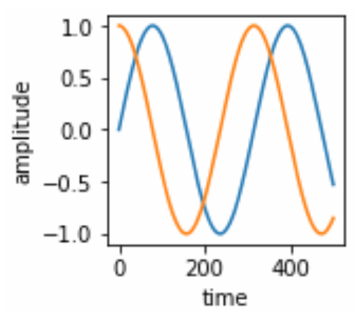
\includegraphics[height=5cm]{./statics/uncorrelated_sine_waves.png}
    \caption{دو سیگنال سینوسی که با هم وابستگی ندارند ولی هر دو در فرکانس یکسانی نوسان می‌کنند}
\end{figure}

برای اندازگیری همبستگی به ازای تمام فازهای ممکن، مانند فازی که باعث می‌شود تا
مقدار همبستگی حداکثر شود، از اعداد موهومی استفاده می‌شود. فرض کنید نقطه‌ای برروی
محور اعداد موهومی از مبدا و در جهت اعداد حقیقی مثبت شروع به حرکت کند. جهت حرکت
این نقطه با با توجه به فرکانس خواسته شده تغییر می‌کنند. همچنین سرعت حرکت این
نقطه در لحظه $t$ برابر با قدرت سیگنال ورودی در  لحظه $t$ است. به عبارتی دیگر،
نقطه یاد شده در زمان $t$ به اندازه قدرت سیگنال ورودی در زمان $t$ و در جهت محاسبه
شده جابه‌جا می‌شود. در پایان فرآیند هرچه نقطه از مبدا دورتر شده باشد، یعنی
وابستگی سیگنال ورودی با سیگنالی سینوسی با فرکانسی برابر فرکانس خواسته شده بیشتر
است. همچنین فازی که باعث بیشتر مقدار وابستگی می‌شود، با جهت کلی حرکت در ارتباط
هست. شکل زیر نمونه‌ای از انجام این فرآیند را برای دو سیگنال مختلف نشان می‌دهد.
مطابق انتظار برای سیگنالی که هم بستگی بسیار پایینی با فرکانس خواسته شده دارد،
نقطه نزدیک مبدا است و برای سیگنالی که همبستگی بیشتری دارد، از مبدا دورتر است.
\begin{figure}[ht]
    \centering
    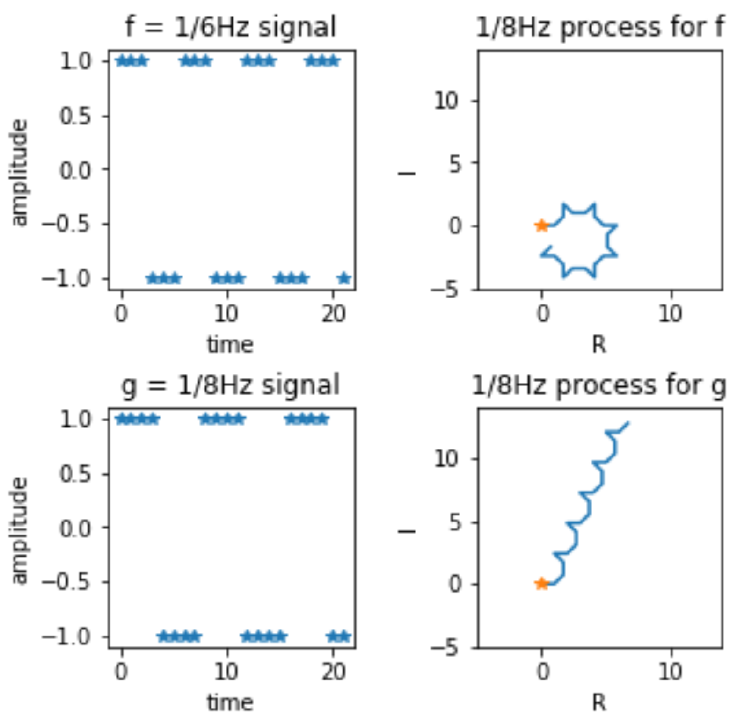
\includegraphics[height=8cm]{./statics/spectral_domain_process.png}
    \caption{انجام فرایند توضیح داده شد بر روی دو سیگنال ورودی مختلف}
\end{figure}

فرایند بالا را می‌توان توسط رابطه زیر مدل کرد:
\begin{equation}
    X(\omega) = \sum_{n} x(n)e^{i \omega \frac{2\pi}{f_s} n}
\end{equation}
که $X(\omega)$ عددی موهومی است که اندازه آن برابر است با میزان حضور یک فرکانس
دلخواه مانند $\omega$ در سیگنال ورودی $x$. همچنین $x(n)$ میزان قدرت سیگنال در در
نمونه $n$ نشان می‌دهد. $e^{i \omega \frac{2\pi}{f_s}}$ برابر جهت حرکت در محور‌
مختصات اعداد موهومی در زمان $t = \frac{n}{f_s}$ است که $f_s$ فرکانس خواسته شد
است. محل توقف نقطه در فرآیند یاد شده همان خروجی این رابطه است که اندازه آن با
میزان حضور فرکانس مطلوب در سیگنال ورودی رابطه دارد.

با کمک رابطه بالا می‌توان می‌توان میزان وجود هر فرکانس در سیگنال ورودی را اندازه
گرفت و در نتیجه سیگنال ورودی را به حوزه فرکانس انتقال داد. حوزه فرکانس میزان
قدرت هر فرکانس در سیگنال ورودی را بیان می‌کند در حالی که حوزه زمان که ابتدا سیگنال
در آن بود قدرت سیگنال در زمان‌های مختلف را مشخص می‌کند.

\subsection{تبدیل فوریه}
معروف‌ترین تبدیل برای انتقال سیگنال از حوزه زمان به حوزه فرکانس تبدیل فرویه هست.
\gls{fft} یک پیاده سازی از این تبدیل است که سیگنال‌هایی که طول آن‌ها توانی از دو
است را می‌توان در $O(nlog(n))$ به حوزه فرکانس ببرد. این تبدیل میزان فعال بودن
فرکانس‌های مختلف را که فاصله خطی از هم دارند را به گونه‌ای محاسبه می‌کند که
سیگنال ابتدایی مجدد بعد از تبدیل قابل محاسبه است. این تبدیل سیگنال ورودی را به
شکل حاصل جمع مجموعه‌ای موج سینوسی با فرکانس‌های مختلف بیان می‌کند. صورت گسسته
این تبدیل که به \gls{dft} معروف است توسط رابطه زیر قابل محاسبه است:
\begin{equation}
    X[k] = \sum_{n=0}^{N-1} x[n]e^{- ikw\omega_0n} \quad \forall k \in \{ 0, 1, ..., N-1 \}
\end{equation}
که $x$ سیگنال ورودی به طول $N$ است و $\omega_0$ برابر $\frac{2\pi}{n}$ است.

همچنین برای بازتولید سیگنال اولیه می‌توان از رابطه زیر استفاده کرد:
\begin{equation}
    x[n] = \frac{1}{N}\sum_{k=0}^{N-1} X[k]e^{ik\omega_0n} \quad \forall n \in \{ 0, 1, ..., N-1 \}
\end{equation}

به صورتی کلی وقتی خروجی تبدیل بررسی می‌شوند تنها اندازه اعداد موهومی به دست آمده
استفاده می‌شود. اندازه این اعداد متناسب با همبستگی سیگنال ورودی با سیگنال‌های
سینوسی بهینه است.

با توجه به سرعت \gls{fft} این تبدیل از حوزه‌های متفاوت به صورت گسترده استفاده
می‌شود. با این وجود در حوزه \gls{mir} این تبدیل یک ضعف مهم دارد. به کمک این
تبدیل می‌توان متوجه شد که یک فرکانس خاص، مثلا ۴۴۰ هرتز، در یک قطعه وجود دارد ولی
راهی برای تشخیص مکان وجود این فرکانس وجود ندارد. یک راه حل برای این ضعف این است
که سیگنال ورودی در فواصل کوتاه برش داده شود و برای هر برش به صورت جداگانه تبدیل
محاسبه گردد. این تبدیل جدید به \gls{stft} معروف است. هرچی فاصله زمانی که برش‌ها
در آن‌ها انجام می‌شود کوتاه‌تر باشد، دقت خروجی در بعد زمان بیشتر است. از طرفی
دیگر کوتاه بودن این فواصل زمانی باعث کاهش دقت در بعد فرکانس می‌شود. خروجی
\gls{STFT} یک نمایش دو بعدی است که یک محور آن نماینده زمان و محور دیگر نماینده
فرکانس است. این نمایش به نمایش زمان-فرکانس معروف است.

\subsection{تبدیل ثابت Q}
یکی از ضعف‌های \gls{stft} در حوزه موسیقی این است که فرکانس‌هایی که وجود آن‌ها در
سیگنال ورودی بررسی می‌شود، فاصله خطی از یک دیگر دارند. این در حالی هست که
\gls{pitch} نت‌های موسیقی در فواصل لگاریتمی از یک دیگر قرار دارند. این تفاوت‌ به
این معنی است که برای نت‌های بم تعداد زیادی فرکانس وجود دارد ولی برای نت‌های
زیرتر فرکانس‌های کمتری وجود دارد.

\gls{cqt} بجای استفاده از فواصل خطی از فواصل لگاریتمی استفاده می‌کند. ایده اصلی
این است که در فرایند توضیح داده شده در ابتدا، فرکانس‌های انتخابی، فاصله‌ای
لگاریتمی نسبت به هم داشته باشند. همچنین این تبدیل به کمک توابع پنجره‌بندی تنها
در بازه‌های زمانی خاصی، وجود فرکانس‌ها را بررسی می‌کند.
\begin{figure}
    \centering
    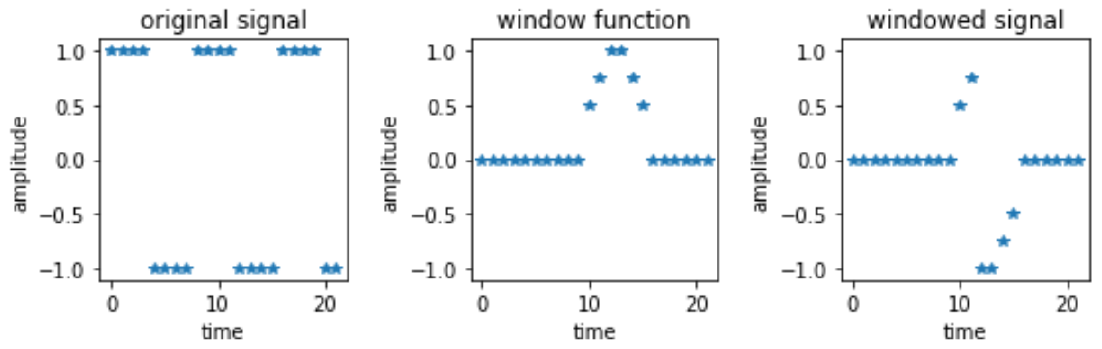
\includegraphics[height=4cm]{./statics/windowed_signal.png}
    \caption{نمونه‌ای از یک سیگنال پنجره‌بندی شده}
\end{figure}

\gls{CQT} را می‌توان به کمک رابطه زیر محاسبه کرد:
\begin{equation}
    X^{CQ}(k, n) = \sum_{j=n-\lfloor N_k / 2 \rfloor}^{n+\lfloor N_k / 2 \rfloor} x(j)a_k^*(j-n+N_k/2) \quad \forall k \in \{1, 2, ..., K \}
\end{equation}
\begin{equation}
    a_k^*(n) = \frac{1}{N_k} w (\frac{n}{N_k}) e^{if_k\frac{2\pi}{f_s}n}
\end{equation}
$X^{CQ}(k, n)$ مقدار خروجی تبدیل برای فرکانس $f_k$ و در اطراف نمونه $n$ سیگنال
ورودی $x$ است. $N_k$ یک عدد حقیقی هست که از پارامترهای تبدیل است. $w$ یک تابع
پنجره‌بندی پیوسته هست که دامنه آن بین صفر و یک است. $f_k$ فرکانس خواسته شده‌
$k$ام است. $f_s$ نیز فرکانسی است که سیگنال ورودی با آن نمونه برداری شده است.

این تبدیل پارامترهای مختلفی دارد که مقدار بهینه آن‌ها با توجه به معیار‌هایی
مانند توانایی باز تولید سیگنال و سرعت محاسبه در \cite{schorkhuber2010constant}
بررسی شده است. در ادامه به بررسی این پارامترها می‌پردازیم.

$f_k$ مقدار فرکانس $k$ام خواسته شده را مشخص می‌کند. با توجه به این که این
فرکانس‌ها با هم فاصله‌ای لگاریتمی دارند، می‌توان مقدار آن‌ها را مقایسه کرد. برای
محاسبه می‌توان از رابطه زیر استفاده کرد:
\begin{equation}
    f_k = f_1 2^{\frac{k-1}{B}} \quad \forall k \in \{1, 2, ..., K\}
\end{equation}
$f_1$ یا $f_{min}$ مقدار پایین‌ترین فرکانس را مشخص می‌کند که سایر فرکانس‌ها از
آن شروع می‌شوند. $B$ مشخص می‌کند به ازای هر اکتاو چند فرکانس انتخاب شود و میزان
حضور آن‌ها در سیگنال ورودی اندازه گرفته شود. همچنین $K$ تعداد کل فرکانس‌های
خواسته شده است. این مقدارها با توجه کاربرد به می‌توانند انتخاب شوند.

$N_k$ عرض پنجره استفاده شده برای فرکانس $k$ام را مشخص می‌کند. مقدار بهینه این
پارامتر را می‌توان با استفاده از رابطه زیر محاسبه کرد:
\begin{equation}
    N_k = \frac{qf_s}{f_k(2^{\frac{1}{b}}-1)} \stackrel{B \geq 12}{\approx} \frac{qf_sB}{log(2)f_k} \quad 0 < q \leq 1
\end{equation}

انجام \gls{cqt} برای هر نمونه نه از نظر محاسبه منطقی است و نه مزیت خاصی دارد. از
این جهت این تبدیل به ازای هر $H_k$ نمونه یک بار انجام می‌شود. مقدار بهینه برای
این پارامتر برابر $\lfloor \frac{1}{2N_k} \rfloor$ است تا تمام طول سیگنال ورودی
پردازش شود. همچنین در عمل معمولا به ازای تمام مقادیر $k$، $H_k = H$ است تا خروجی
را بتوان به شکل یک ماتریس نمایش داد.

$w$ تابع پنجره‌بندی مورد استفاده است که به صورت سنتی از تابع $Hann$ برای آن
استفاده می‌شود. این تابع برشی از تابع سینوس‌ هست که در زیر نمودار آن نشان داده شده
است.
\begin{figure}[ht]
    \centering
    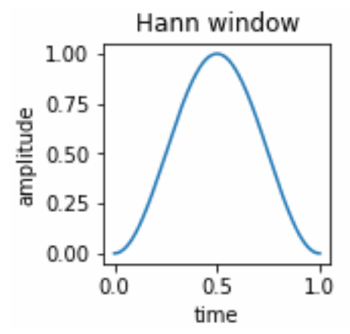
\includegraphics[height=5cm]{./statics/hann_plot.png}
    \caption{نمودار تابع پنجره‌بندی Hann}
\end{figure}

در نهایت $f_s$ فرکانس نمونه‌برداری از سیگنال اولیه است. برای صحت محاسبات رابطه
زیر باید برقرار باشد:
\begin{equation}
    f_s \geq 2f_k
\end{equation}

\subsection{اسپکتروگرام mel}
با توجه به این که درک انسان از صوت یک درک کاملا لگاریتمی نیست، مقیاس دیگری برای
انجام آزمایشات ساخته شده است که به مقیاس mel معروف است. با وجود این که بیش از یک
مقیاس mel ساخته شده، ولی تمام آن‌ها تنها تفاوت‌هایی جزئی با هم دارند. در این
پایان‌نامه فقط یکی از این مقیاس‌ها توضیح داده شده است که همان مقیاسی است که در
این پایان‌نامه استفاده شده است و کتابخانه librosa آن را پیاده‌سازی کرده است
\cite{mcfee2015librosa}.

آزمایشات انجام شده بر روی شنوایی انسان نشان داده‌اند که درک انسان از صوت، تا
هزار هرتز، یک درک خطی است. برای اصوات بالای هزار هرتز این درک به شکل لگاریتمی در
می‌آید. با این توصیف رابطه زیر می‌تواند این مقیاس را مدل کند:
\begin{equation}
    x Hz =
    \begin{cases}
        \frac{3x}{200}mel &\quad x \leq 1000\\
        15 + 27 ln(x/1000) / ln(6.4) mel &\quad \text{elsewhere}
    \end{cases}
\end{equation}

کتاب‌خانه librosa \gls{spec} با مقیاس mel را به کمک رابطه زیر محاسبه می‌کند:
\begin{equation}
    X^{MEL}(k, n) = \sum_{j=0}^{n_{fft}-1} |X_n|^2(j)A_k^*(\frac{f_s}{n_{fft}}j)
\end{equation}
$|X_n|$ اندازه \gls{dft} سیگنال ورودی $x$ در اطراف $n$ با $n_{fft}$ نمونه است.
$A_k^*$ یک تابع پنجره‌بندی از اعداد حقیقی به اعداد حقیقی است. این تابع شکلی
مثلثی دارد و در $f_{k-1}$ مقدار صفر دارد. در $f_k$ به $V_{max}^{k}$ می‌رسد و
مجددا در $f_{k+1}$ صفر می‌شود. $V_{max}^{k}$ به گونه‌ای مقدار داده می‌شود که
تقریبا برای هر کانال مقداری ثابت داشته باشد. این مقدار از رابطه زیر به دست
می‌آید:
\begin{equation}
    V_{max}^{k} = \frac{2}{f_{k+1} - f_{k-1}}
\end{equation}
$\frac{f_s}{n_{fft}}j$ فرکانس متناظر با $j$امین فرکانس استفاده شده در \gls{dft}
است. همچنین $f_s$ فرکانس نمونه‌گیری سیگنال ورودی $x$ است.

\subsection{قالب فرکانسی یک نت}
وقتی که صوت حاصل از اجرای یک نت تنها، از حوزه زمان به خوزه فرکانس انتقال داده
شود، \gls{spec} به دست آمده، قالب فرکانس آن نت نامیده می‌شود. وقتی که

در شکل زیر قالب فرکانسی نت $A5$ که بر روی ساز پیانو اجرا شده است رسم شده است.
همچنین فرکانس‌ها با یک دیگر فاصله‌ای لگاریتمی دارند تا متناظر با \gls{pitch}
نت‌های پیانو باشند. همچنین که در \gls{spec} رسم شده کاملا واضح است، علاوه بر
فرکانس پایه نت، فرکانس‌های پایه‌ای دیگری نیز کامل در صوت تولید شده حضور دارند.
این فرکانس‌ها با خط سفید مشخص شده‌اند. این پدیده رفتاری کاملا انتظار از یک ساز
موسیقی است و یکی از عوامل اصلی سختی مسئله \gls{atm} محسوب می‌شود. همچنین این
رفتار وجه اصلی تمایز مسئله \gls{asr} با مسئله \gls{atm} است. این فرکانس‌‌های
فعال، به عنوان هامونیک‌های نت نواخته شده شناخته می‌شود. با توجه به این که این
هامونیک‌ها خود متناظر با نت‌های دیگری نیز هستند که احتمال نواخته شدن بالایی نیز
با نت پایه دارند، تشخیص نت‌های فعال را بسیار پیچیده می‌کنند.

همچنین، با توجه به شکل کاملا واضح است که در لظحه نواخته شدن نت، فرکانس‌های فعال
دیگری نیز در صوت تولید شده حضور دارند. دلیل حضور این فرکانس‌ها این است که وقتی
یک سیم پیانو توسط چکش نواخته می‌شود، در لحظه شروع حجم زیادی نویز تولید می‌کند که
باعث حضور بازه گسترده‌ای از فرکانس‌ها می‌شود. ولی پس از گذشت زمانی کوتاه، سیم
شروع می‌کند به در فرکانس متناظر نوسان کردن و فرکانس‌های اضافه حذف می‌شوند. حضور
این بازه گسترده از فرکانس‌ها باعث می‌شود که شروع نت‌ها به شکل بسیار ساده‌تری
قابل تشخیص باشد.
\begin{figure}[ht]
    \centering
    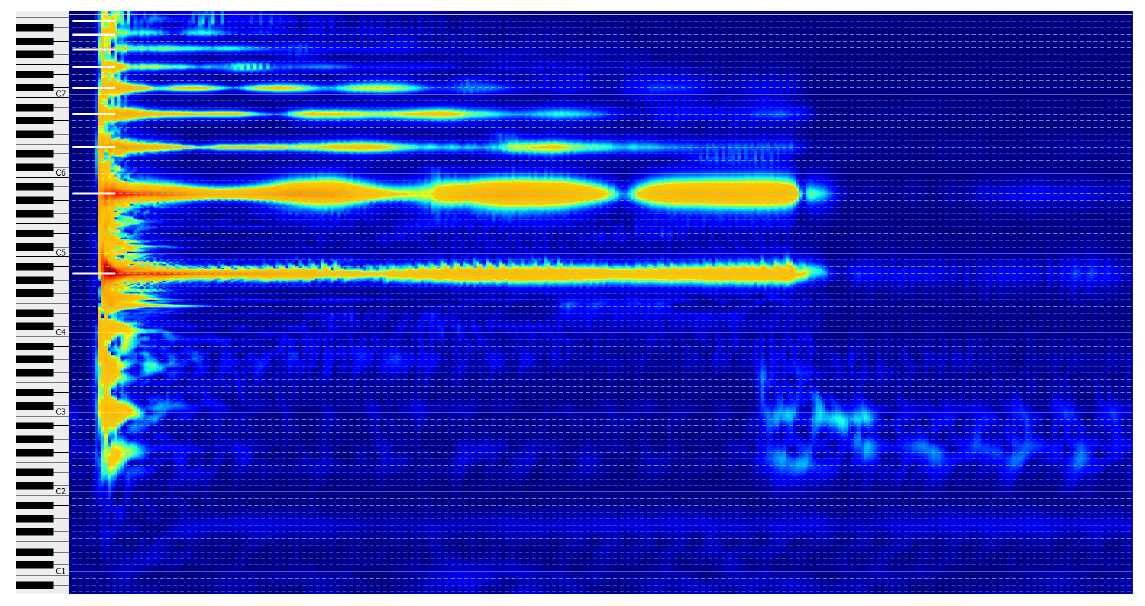
\includegraphics[width=15cm]{./statics/a5_spec.png}
    \caption{\gls{spec} متناظر با نواخته شدن نت A5 بر روی پیانو}
\end{figure}

\section{یادگیری ژرف}
در سال‌های اخیر، \gls{ml} روز به روز محبوب‌تر شده‌است در برای حل مسائلی مانند
دسته‌بندی تصاویر، پیشنهاد ویدیو، تحلیل شبکه‌های اجتماعی و پردازش متن به صورت
گسترده استفاده می‌شود. در میان روش‌های \gls{ml}، \gls{dl} موفقیت‌های بسیاری برای
حل این مسائل و مسائل دیگر به دست آورده است. رشد نمایی داده و پیشرفت‌های
سخت‌افزاری باعث شده که تحقیقات گسترده‌ای بر روی \gls{dl} صورت بپذیرد. \gls{dl}
که پیدایش آن ریشه در \gls{nn} دارد، توانسته به خوبی از پدران خود پیشه بگیرد و
نتایج بسیاری بهتری به دست بیاورد. روش‌های اخیر در \gls{dl} نتایج بسیار امیدوار
کننده‌ای در حوزه‌های پردازش تصویر، گفتار و زبان طبیعی به دست آورده‌اند و در خیلی
از مسائل انسان حتی پیشه گرفته‌اند.

به صورت سنتی، نمایشی که برای برای داده انتخاب می‌شود، تاثیر به سزایی در دقت
نهایی سیستم دارد و یک نمایش نامناسب از داده باعث دقت به‌شدت پایین‌تری می‌شده
است. از این جهت بررسی شیوه‌های موثر نمایش داده، در \gls{ml}، از چالش‌های اصلی
حوزه محسوب می‌شده است و مطالعات زیادی بر روی آن‌ها انجام شده است. با این وجود
این یافته‌ها اکثرا تنها محدود به حوزه خاصی هستند و قابل تعمیم به سایر حوزه‌ها
نیستند.

در مقابل، در \gls{dl}، تمام این فرایند استخراج ویژگی از داده‌های ورودی و تبدیل
آن‌ها به نمایشی مناسب، به صورت خوکار، توسط مدل فراگرفته و اعمال می‌شود. این
ویژگی این خانواده از مدل‌ها باعث می‌شود که نیاز به دخالت متخصص حداقل شود و
سیستم‌هایی کارا، بدون نیاز دانش حوزه، طراحی شوند.

سیستم‌های مبتنی بر \gls{dl} شامل مجموعه‌ای از لایه‌های غیرخطی هستند که می‌توانند
اطلاعات را در ساختاری سلسله‌مراتبی استخراج کنند. لایه‌های ابتدایی مدل، مسئول
استخراج ویژگی‌های سطح پایین‌تر هستند. سپس لایه‌های بعدی از این ویژگی‌های استخراج
شده استفاده می‌کنند تا ویژگی‌های سطح بالاتری را استخراج کنند. این دقیقا همان
رفتاری است که مغز انسان برای پردازش داده‌های ورودی و تصمیم‌گیری بر اساس آن‌ها
انجام می‌دهد. برای مثال در سیستم بینایی انسان، نرون‌های ابتدایی تنها وظیفه
استخراج نقطه‌ها را دارند. از موقعیت نقطه‌های استخراج شده استفاده می‌شود تا خطوط
تشخیص داده شوند. به همین شکل مغز اشکال پیچیده‌تر را پیدا می‌کند و تشخیص می‌دهد
در لحظه در حال مشاهده چه اجسامی می‌باشد.

\subsection{تاریخچه یادگیری ژرف}
ساختن ماشینی که مشابه مغز انسان کار کند و بتواند مانند مغز مسائل را حل کند
رویایی به قدمت چندین قرن برای دانشمندان است با این حال شروع تاریخجه مدرن
\gls{dl} را می‌توان از ۱۹۴۳ دانست که \lr{McCulloch-Pitts} معرفی شد. این مدل
اولین مدل ساختار نرون محسوب می‌شود و نمونه‌ای اولیه از \gls{nn} امروزی است. مدل
معرفی شده می‌توانست تا حدی رفتار یک نرون مغزی را مدل کند ولی هیچ قاعده‌ای برای
یادگیری معرفی شد. از آن زمان \gls{dl} به آرامی شروع به پیداش و پیشرفت کرد و طی
چندین رخداد مهم تبدیل به ساختار امروزی شد.

پس از معرفی مدل \lr{McCulloch-Pitts} قاعده یادگیری هب معرفی شد که ریشه‌ای زیستی
دارد و برای آموزش شبکه‌های اولیه استفاده می‌شود. سپس در سال ۱۹۵۸ در حوزه علوم
شناختی، مدل پرسپترون معرفی شد که ساختاری بسیار نزدیک به \gls{nn} امروزی دارد. با
پایان یافتن دوره رکود اولی \gls{ai}، پیدایش \gls{backpropagation} رخداد تارخی
مهم بعدی در پیدایش \gls{dl} بود. به کمک \gls{backpropagation} آموزش \gls{nn} به
کمک یک تابع خطا ممکن شد. در سال ۱۹۸۰ neocogitron معرفی شد که منجر به پیدایش
\gls{cnn} شد. همچنین در سال ۱۹۸۶ با معرفی \gls{rnn} امکان پردازش داده‌های
دنباله‌ای محقق شد. در نهایت در ده ۹۰ میلادی با معرفی LeNet اولین شبکه عصبی عمیق
معرفی شد. هرچند این شبکه در زمان انتشار، به علت محدودیت‌های سخت‌افزاری به شهرت
زیادی دست نیافت.

در ۲۰۰۶ \gls{dbn} همراه با یک شیوه آموزش لایه به لایه معرفی شدند. ایده اصلی این
شبکه‌ها این بود که یک شبکه دولایه ساده با \gls{unsupervised learning} و مشابه
\gls{rbm} آموزش داده شود. سپس تمام پارامترهای فراگرفته شده قفل شوند، یک لایه
جدید در ادامه شبکه قرار داده شود، و پارامترهای این لایه همچون لایه قبل فراگرفته
شود. با کمک این شیوه آموزش، محققان توانستند شبکه‌هایی با عمق به شدت بیشتر از
مدل‌های قبلی را آموزش دهند. \gls{dl} بعد از سال‌ها توسعه و با ریشه در \gls{nn}
یکی از روش‌های پرطرفدار در \gls{ml} محسوب می‌شوند که توانسته است موفقیت‌های
زیادی به دست آورد.

از موفقیت‌های اخیر \gls{dl} می‌توان از AlphaGo نام برد که در ابتدای ۲۰۱۷ توسط
تیمی از گوگل معرفی شد و با عملکرد خود دنیا را متعجب ساخت. این مدل توانست تحت نام
مستعار master، ۶۰ بازی Go در مقابل حریفان حرفه‌ای برنده شود. از جمله این
پیروزی‌ها سه برد پیاپی در مقابل \lr{Ke Jie} است. این شبکه توانست با بهره‌گیری از
روش‌های مدرن \gls{dl} و سخت‌افزاری قدرتمند برای آموزش، قهرمان چهانی این بازی را
شکست دهد.

\subsection{شبکه‌های عصبی مصنوعی}
شبکه‌های عصبی مصنوعی سیستم‌های محاسباتی هستند که از شبکه‌های عصبی زیستی الهام
گرفته‌اند. این سیستم‌ها از طریق مشاهده مثال‌ها و بدون نیاز به برنامه‌ریزی مستقیم
می‌توانند مسائل مختلفی را حل کنند. برای مثال این شبکه‌ها با دیدن تصاویر زیادی که
حاوی ماشین بوده‌اند، در تصاویر جدید ماشین را، بدون نیاز به تعریف مستقیم ماشین،
تشخیص دهند. از این جهت از شبکه‌های عصبی مصنوعی در حل مسائلی که نمی‌توان به راحتی
از طریق الگوریتم‌های قانونمند برای حل آن‌ها اقدام کرد، استفاده می‌شود.

یک شبکه عصبی مصنوعی از تعداد زیادی واحدهای کوچک‌تر که یک نرون مصنوعی نامیده
می‌شوند تشکیل شده است. این نرون‌ها توسط اتصالاتی به نام سیناپس به یکدیگر مرتبط
اند که می‌تواند سیگنال‌ها را از نرونی به نرون بعدی منتقل کند. به این طریق هر
نرون می‌تواند مجموعه‌ای از سیگنال‌های ورودی را گرفته، آن‌ها را پردازش کند و از
طریق سیگنالی نتیجه را به نرون‌های بعدی منتقل کند. همچنین این سیناپس‌ها معمولا
دارای وزن‌هایی می‌باشند که میزان اهمیت یک سیگنال برای نرون دریافت کننده آن را
نشان می‌دهد و فرآیند یادگیری شامل تنظیم این وزن‌ها است.

به طور معمول نرون‌ها به شکل لایه لایه قرار داده می‌شنود که هر لایه عمل مخصوص به
خود را انجام می‌دهد و نتیجه را به لایه بعد منتقل می‌کند. برای مثال شبکه‌ای را در
نظر بگیرید که هدف آن تشخیص اشیای مختلف باشد. این شبکه از لایه‌های مختلفی تشکیل
شده است. در فرآیند یادگیری ممکن است این لایه اول نسبت به خطها حساس شده باشد.
یعنی هر نرون این لایه در صورت وجود خطی با زاویه و ضخامتی مشخص و در جایی مشخص از
تصویر، سیگنال‌های شدیدتری به لایه بعدی ارسال کند. حال لایه بعد می‌تواند از
اطلاعات ارسالی از لایه قبل استفاده کرده، و با توجه به اطلاعات خطها شکل‌های هندسی
ساده را تشخیص دهد.

هدف اصلی شبکه‌های عصبی مصنوعی پردازش اطلاعات و حل مسائل به همان شیوه‌ای بود که
مغز انسان مسائل را حل می‌کند. ولی در طول زمان با تمرکز بروی مسائل مختلف باعث شد
عملکردهایی اضافه شوند که گاها هیچ توجیح زیستی‌ای ندارند. به عنوان نمونه می‌توان
به فرآیند پس‌انتشار خطا اشاره کرد که با این که هیچ ریشه زیستی ندارند ولی یکی از
اصلی‌ترین شیوه‌های آموزش شبکه‌های عصبی عمیق محسوب می‌شود.

با گذر زمان و افزایش توان محاسباتی کامپیوترها، دانشمندان توانستند شبکه‌های عصبی
بزرگ‌تر و پیچیده‌تری طراحی کنند و با استفاده از آن‌ها مسائل سخت‌تری را حل
نمایند. در حال حاضر هر شبکه ممکن است تا حدود چند میلیون نرون داشته باشد. با این
حال هنوز تا شبکه‌هایی به پیچیدگی مغز انسان که راه بسیاری باقی مانده است.

\subsection{روش‌های یادگیری}
روش‌های \gls{dl} را می‌توان به سه دسته \gls{supervised learning}،
\gls{unsupervised learning} و \gls{semisupervised learning} تقسیم کرد. همچنین
\gls{reinforcement learning} نیز دسته دیگری از روش‌ها را شامل می‌شود که خود زیر مجموعه‌ای از
روش‌های \gls{semisupervised learning} است.

\gls{supervised learning} روش‌هایی هستند که از برچسب داده‌گان برای آموزش استفاده
می‌کنند. در این خانواده از روش‌ها دادگان به شکل زوج مرتب $(x, y)$ هستند که $x$
ورودی مدل است و $y$ خروجی مورد نظر است. در صورتی که مدل به ازای ورودی $x$ مقدار
$y^{\prime}$ را برگداند، مقادیر $y$ و $y^\prime$ به یک تابع خطا، مثلا $L$، داده
می‌شوند و پارامترهای مدل به گونه‌ای تغییر داده می‌شود که مقدار $L(y, y^\prime)$
کاهش یابد. پس از پایان آموزش انتظار می‌رد که در صورتی که ورودی $x$ به مدل داده
شود، مدل بتواند جواب درست، $y$ را تشخیص دهد و برگرداند.

\gls{unsupervised learning} به روش‌هایی گفته می‌شود که داده‌گان مورد آموزش در
آن‌ها دارای برچسب نمی‌باشد. در این روش‌ها مدل تلاش می‌کند تا ساختار داخلی یا
ویژگی‌های مهم ورودی را فراگیرد و با کمک آن‌ها روابط بین داده‌گان ورودی را
پیدا کند. \gls{clustering} و \gls{dimensionality reduction} نمونه‌هایی از مسائل
\gls{unsupervised learning} محسوب می‌شوند.

\gls{semisupervised learning} به روش‌هایی اطلاق می‌شود که تنها بخشی از دادگان
آموزش آن‌ها دارای برچسب هستند. در این روش‌ها معمولا بخشی از مدل توسط روش‌های
\gls{unsupervised learning} و بخش دیگر توسط روش‌های \gls{supervised learning}
آموزش داده می‌شود.

\subsection{طراحی و آموزش شبکه‌ها عصبی عمیق}
طراحی شبکه‌های عصبی شامل تعیین تعداد لایه‌ها، نوع و اندازه هر لایه، شیوه ارتباط
لایه‌ها و تابع خطا با توجه ماهیت مسئله مورد نظر است. این پارامترها که ساختار مدل
را مشخص می‌کنند با نام \gls{hyper parameter} شناخته می‌شوند.

فرض کنید یک شبکه عصبی یک تابع هست که می‌خواهد تقریبی از تابع $f$ از $X$ به $Y$
باشد. نمونه‌هایی از مقادیر $X$ و مقدار متناظر آن‌ها در $Y$ به شکل \gls{dataset}
آموزش داده شده‌اند. ساختار استفاده شده برای شبکه، شکل این تابع مشخص می‌کند و
محدودیتی بر روی ساختار آن اعمال می‌کند. از این جهت در زمان طراحی تلاش می‌شود تا
ساختار به گونه‌ای انتخاب شود که محدودیت‌های اعمال شده مانع انعطاف پذیری مورد
نیاز تابع نشوند و تابع ظرفیت کافی برای تقریبی مناسب را دارا باشد. همچنین تابع
انعطاف پذیری بیشتر از مقدار مورد نیاز نیز نداشته باشد تا منجر به \gls{overfit}
نشود.

پس از طراحی، وزن‌های شبکه به عنوان پارامترهای شبکه محسوب می‌شوند. به عبارتی دیگر
خروجی شبکه، $y^\prime$، به صورت تابعی از ورودی شبکه، $x$، و وزن‌های شبکه، $w$
است. در این مرحله با معرفی تابع خطا، $J(w)$، تفاوت بین مقدار خروجی شبکه،
$y^\prime$ و مقدار مورد نظر، $y$، اندازه گرفته می‌شود. این تابع خطا به گونه‌ای
انتخاب می‌شود که کاهش مقدار آن به معنای نزدیک شدن شبکه به تابعی که قصد تقریب آن
را داشتیم باشد تا مسئله حل شود.

آموزش شبکه یک فرآیند تکرار شونده از تنظیم وزن‌های شبکه، $w$، به گونه‌ای است که
مقدار تابع خطا، $J(w)$، کاهش یابد. تابع خطا یک روش برای ارزیابی خروجی‌های شبکه
با توجه مقدار درست آن‌ها است. یک روش مناسب برای کاهش مقدار تابع خطا استفاده از
\gls{backpropagation} و \gls{gd} است که در هر مرحله مقدار وزن‌های شبکه، $w$، را
به شکلی تغییر می‌دهد که مقدار تابع خطا، $J(w)$، بیشترین کاهش را داشته باشد.
\gls{gd} را توسط رابطه زیر می‌توان مدل کرد:
\begin{equation}
    w := w - \eta \nabla J(w)
\end{equation}
که $\eta$ نرخ یادگیری و $\nabla J(w)$ گرادیان $J(w)$ هستند. همچنین برای محاسبه
گرادیان $J(w)$ از الگوریتم \gls{backpropagation} استفاده می‌شود که با استفاده از
قاعده زنجیره‌ای مشتق در هر لایه گرادیان را محاسبه می‌کند.

سرعت آموزش شبکه تاثیر به شدت بالایی بر روی دقت نهایی سیستم دارد. دلیل این امر
این است که اگر دو شبکه با سرعت خیلی تفاوتی آموزش داده شوند، ممکن است در نقاط
مختلفی همگرا شوند و در نتیجه تفاوت زیادی در دقت نهایی داشته باشند. همچنین اگر
سرعت یادگیری از حد بیشتر شود، ممکن است شبکه حتی همگرا نشود و دقت حتی کاهش پیدا
کند. با توجه به رابطه بالا مشخص است که نرخ یادگیری و گرادیان $J(w)$ دو عاملی
هستند که موفقیت آموزش شبکه به آن‌ها بستگی دارد.

نرخ یادگیری می‌تواند به صورت پویا در طول فرآیند یادگیری تغییر داده شود. معمولا
نرخ یادگیری در ابتدای آموزش مقداری بالا دارد. هرچی آموزش شبکه پیش می‌رود، نرخ
یادگیری کاهش پیدا می‌کند. با این شیوه یادگیری، در ابتدای تغییرات وزن‌ها بیشتر
است و هرچی شبکه بیشتر به سمت همگرایی پیش برود، با کاهش نرخ یادگیری، تغییرات کمتر
می‌شود و شبکه با دقت بیشتری همگرا می‌شود. در سال‌های اخیر ADAM یکی از روش‌های
محبوب برای آموزش \gls{nn} است که به صورت خودکار تنظیم نرخ یادگیری را انجام
می‌دهد \cite{kingma2014adam}.

گرادیان تابع خطا نیز تاثیر به شدت زیادی در آموزش شبکه دارد. با توجه به شیوه کار
الگوریتم \gls{backpropagation}، گرادیان هر لایه تاثیر مستقیمی بر روی گرادیان
لایه‌های قبلی دارد. در نتیجه در صورتی که گرادیان‌ها در طول شبکه به صورت مناسبی
جریان نداشته باشند، آموزش شبکه با مشکلات جدی مواجه می‌شود و معمولا لایه‌های
ابتدایی آموزش صحیحی را دریافت نمی‌کند. موفقیت ساختارهایی مانند \gls{lstm} و
ارتباطهای رزیدوال که دقیقا با هدف جریان بهتر گرادیان‌ها طراحی شده‌اند، شاهدی بر
اهمیت این موضوع است.

توابع فعال‌سازی که در هر لایه استفاده می‌شود یکی دیگر از نکاتی هست که نیاز به
توجه بالا دارند. این توابع با معرفی کردن عاملی غیر خطی بین لایه‌ها به شبکه این
قابلیت را می‌دهند که الگوهای بسیار پیچیده‌تری را بتواند فرا بگیرد. همچنین این
توابع بر روی جریان گرادیان‌ها نیز تاثیر قابل توجهی دارند.

دو تا از توابع فعال‌سازی که به صورت گسترده، مخصوصا تا اوایل دهه‌ي ده میلادی،
استفاده می‌شود تابع سیگموید و تابع  تانژانت هیپربولیک است که در روابط زیر ضابطه
آن‌ها نشان داده شده است:
\begin{equation}
    sig(x) = \frac{1}{1 + e^{-x}}
\end{equation}
\begin{equation}
    tanh(x) = \frac{e^x - e^{-x}}{e^x + e^{-x}}
\end{equation}

با این وجود شبکه‌هایی که از این شبکه‌ها استفاده می‌کنند ممکن است از مشکل محو شدن
گرادیان در لایه‌های ابتدایی رنج ببرند \cite{bengio1994learning}. محو شدگی
گرادیان به شرایط گفته می‌شود که گرادیان تابع خطا در بخش‌هایی از شبکه مقداری
نزدیک به صفر پیدا کند. در نتیجه آن بخش‌های شبکه تقریبا هیچ آموزشی دریافت
نمی‌کنند یا آموزشی اشتباه دریافت می‌کنند.

برای حل این معضل، تابع فعال ساز ReLU پیشنهاد شد \cite{glorot2011deep}. این تابع
در سال‌های اخیر به عنوان تابع فعال‌ساز در اکثر فعالیت‌های منتشر شده استفاده شده
است. همچنین برای حل مشکل تغییر نکردن وزن نرون‌های غیر فعال تابع \lr{Leaky ReLU}
به عنوان یک جایگزین معرفی شد. در شکل زیر نمودار این چهار تابع فعال‌سازی رسم شده
است.
\begin{figure}[ht]
    \centering
    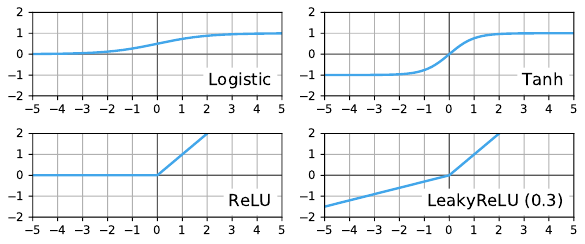
\includegraphics[width=12cm]{./statics/activation_functions.png}
    \caption{نمودار توابع فعال‌سازی معرفی شده}
\end{figure}

به عنوان تابع فعال‌سازی لایه آخر توصیه می‌شود از تابعی استفاده شود که بردی برابر
با بازه برچسب‌های \gls{dataset} داشته باشد. برای مثال اگر خروجی از جنس احتمال
است، تابع فعال‌سازی سیگموید که بردی آن بین صفر و یک است انتخاب مناسبی است. اگر
مسئله \gls{classification} با چند دسته است، تابع softmax توصیه می‌شود. این تابع
فعال سازی می‌تواند به ازای هر نرون خروجی، گرادیان مناسب را تولید کند. اگر مسئله
\gls{regression} است که خروجی محدودیتی ندارد استفاده از یک تابع فعال‌ساز خطی
توصیه می‌شود.

\subsection{تابع خطا}
آموزش در \gls{nn} با کمک تابع خطا رخ می‌دهد. با استفاده از تابع خطا می‌توانیم
توانایی شبکه در حل مسئله مورد نظر را ارزیابی کنیم. وقتی که مدل بتواند خروجی‌های
مناسب را به ازای ورودی‌های داده شده تولید کند، مقدار تابع خطا پایین خواهد بود.
هرچی که خروجی مدل از مقدار مورد نظر کمتر باشد، مقدار تابع خطا افزایش پیدا
می‌کند. پس در صورتی که ابزاری برای کاهش مقدار تابع خطا داشته باشیم می‌توان
جواب‌های درست به ازای ورودی‌های مختلف را به مدل آموزش دهیم. همچنین از مقدار تابع
خطا بر روی کل \gls{dataset} می‌توان استفاده کرد تا توانایی مدل‌های مختلف بر
مسئله مورد نظر را با هم مقایسه کنیم.

توابع خطا بسیار زیادی پیشنهاد شده‌اند که باید با توجه به ماهیت مسئله مورد هدف و
ساختار شبکه استفاده شده، تابع مناسب را از بین آن‌ها انتخاب کرد. به صورت کلی
توابع خطا را به دو دسته بزرگ می‌توان تقسیم کرد. توابع خطا مسائل
\gls{classification} و توابع خطا مسائل \gls{regression}. مسائل
\gls{classification} مسائلی هستند که در آن‌ها هدف اختصاص یک یا چند برچسب به
ورودی داده شده است. تابع Hinge و \gls{cross entropy} نمونه‌ای از توابع خطا مناسب
برای مسائل \gls{classification} هستند. مسائل \gls{regression} مسائلی هستند که در
آن‌ها هدف اختصاص یک یا چند مقدار عددی به ورودی داده شده است. \gls{mse} نمونه‌ای
از یک تابع خطا برای مسائل \gls{regression} است.

تابع \gls{cross entropy} محبوب‌ترین تابع خطا برای مسائل \gls{classification}
محسوب می‌شود. مقدار این تابع خطا بر اساس احتمال پیشبینی شده برای هر برچسب و
برچسب‌های صحیح هر نمونه محاسبه می‌شود و توسط رابطه زیر می‌توان آن را محسابه کرد:
\begin{equation}
    CrossEntropyLoss(y, y^\prime) = \sum_{c=1}^{M} y_i log(y_i^\prime)
\end{equation}
$M$ نشان دهنده تعداد برچسب‌های مختلف مسئله است که هر ورودی مطلق به یکی از آن‌ها
هست. $y_i$ نشان دهنده اختصاص برچسب $i$ به ورودی است. در صورتی که ورودی متعلق به
این گروه باشد، مقدار آن یک است. در غیر این صورت مقدار آن صفر است. همچنین
$y_i^\prime$ احتمال محاسبه توسط مدل برای برچسب $i$ است. معمولا از softmax به
عنوان تابع فعال سازی همراه این تابع خطا استفاده می‌شود.

در صورتی که تنها دو بر چسب مثبت و منفی داشته باشیم و بخواهیم احتمال یک خصوصیت در
ورودی را پیشبینی کنیم، از رابطه ساده شده زیر می‌توان استفاده کرد:
\begin{equation}
    BinaryCrossEntropyLoss(y, y^\prime) = -(y log(y^\prime)) + (1 - y)log(1 - y^\prime)
\end{equation}
sigmoid تابع فعال‌سازی است توصیه شده برای این تابع خطا است.

\gls{mse} یکی از توابع خطای محبوب برای مسائل \gls{regression} محسوب می‌شود. این
تابع خطا فاصله اقلیدوسی بین نقطه پیشبینی شده توسط شبکه و نقطه مورد هدف را محاسبه
می‌کند در نتیجه هرچی خروجی شبکه نامناسب‌تر باشد، مقدار تابع خطا بیشتر می‌شود.
مقدار خطا توسط رابطه زیر قابل مقایسه است:
\begin{equation}
    MSE(y, y^\prime) = \frac{1}{M} \sum_{c=1}^{M} (y_i - y_i^\prime)^2
\end{equation}
که $M$ اندازه ابعاد فضای خروجی است و $y^\prime$ نقطه پیشبینی شده توسط شبکه است.
همچنین $y$ نقطه هدف مورد نظر است.

\subsection{الگوریتم پس‌انتشار خطا}
\gls{backpropagation} یک روش برای محاسبه گرادیان تابع خطا نسبت به وزن‌های
سیناپس‌ها در شبکه‌های عصبی مصنوعی است. این روش معمولا به همراه یک الگوریتم
بهینه‌سازی، مانند \gls{gd}، به عنوان الگوریتم آموزش شبکه‌های عصبی مصنوعی به کار
گرفته می‌شود. هرچند معمولا به کل الگوریتم آموزش استفاده شده پس انتشار خطا گفته
می‌شود ولی در عمل، پس انتشار خطا تقریبا همان قاعده زنجیره‌ای مشتق است و تنها
وظیفه محاسبه گرادیان را بر عهده دارد.

الگوریتم بهینه سازی معمولا شامل دو گام است که متوالیا و به صورت پی‌در‌پی تکرار
می‌شوند: محاسبه گرادیان و بروزرسانی وزن‌ها. وقتی که یک بردار ورودی به شبکه داده
می‌شود، سیگنال‌های خروجی لایه‌ها به ترتیب محاسبه می‌شود تا خروجی آخرین لایه شبکه
به دست آید. به این مرحله \gls{feedforward} گفته می‌شود. سپس مقدار لایه آخر با
مقدار دلخواه ما مقایسه می‌شود و با توجه به اختلاف آن‌ها یک مقدار خطا محاسبه
می‌شود. سپس از این خطا نسبت به وزن‌های لایه آخر گرادیان گرفته می‌شود و این مقدار
گرادیان با توجه به قاعده زنجره‌ای مشتق به لایه‌های قبل منتقل می‌شود و سهم هر
سیناپس در مقدار خطا محاسبه می‌شود. این مرحله \gls{backpropagation} نام دارد. در
نهایت گرادیان محاسبه شده به الگوریتم بهینه‌سازی داده می‌شود تا وزن جدید هر
سیناپس محاسبه شود.

در طی فرآیند آموزش هر نرون یاد می‌گیرد طوری وزن‌های خود را تغییر دهد که نرون‌های
مختلف نشان دهنده خصوصیت‌های مختلفی از ورودی شبکه‌ باشد. وقتی که آموزش شبکه به
پایان رسید، وقتی ورودی که حاوی الگویی است که یک نرون شبکه به آن حساس شده است، به
شبکه داده می‌شود، آن نرون از خود فعالیت بیشتری نشان می‌دهد.

همان گونه که گفته شد برای محاسبه مقدار خطا در این روش نیاز به دانستن خروجی مطلوب
شبکه در مرحله آموزش است. به این جهت روش آموزش \gls{backpropagation}، معمولا یک
روش \gls{supervised learning} محسوب می‌شود هر چند در معماری‌هایی همچون
\gls{autoencoder}، از این الگوریتم برای آموزش بدون نظارت استفاده می‌شود.

هرچند که در تئوری لازمه این روش این است که توابع فعال‌ساز استفاده شده در شبکه
توابعی مشتق‌پذیر باشند، ولی در عمل توابعی همچون ReLU که در یک یا چند نقطه از
دامنه خود مشتق پذیر نیستند هم می‌توان استفاده کرد.

\subsection{الگوریتم‌های بهینه‌سازی}
آموزش شبکه‌های عصبی در اصل یک فرایند بهینه‌سازی است که طی آن تلاش می شود وزن‌های
شبکه به گونه‌ای تنظیم شوند که مقدار تابع خطا کمینه شود. در عمل \gls{sgd}
الگوریتم پایه‌ای است که برای آموزش شبکه‌های عصبی از آن استفاده می‌شود. این
الگوریتم به صورت پی‌درپی وزن‌های شبکه را با توجه به یک نمونه از \gls{dataset} به
گونه‌ای تغییر می‌دهد که مقدار تابع خطا کاهش پیدا کند. همچنین بار محاسباتی
\gls{sgd} در مقایسه با \gls{gd} که کل \gls{dataset} را در هر مرحله در نظر
می‌گرد به شدت کمتر است.

در طی فرآیند یادگیری میزان تاثیر هر مرحله توسط نرخ یادگیری کنترل می شود. نرخ
یادگیری پایین‌تر باعث می‌شود که درنهایت شبکه به نقطه‌ای بهینه‌تر همگرا شود در
حالی که زمان آموزش را به شدت افزایش می‌دهد. نرخ یادگیری بالاتر باعث می‌شود که
سرعت کاهش خطا بیشتر شود ولی ممکن است فرآیند یادگیری را بی‌ثبات کند و مانع همگرا
شدن شبکه شود. برای کنترل نوسانات \gls{SGD} پیشنهاد شد که از مفهوم \gls{momentum}
استفاده شود. \gls{momentum} که از قانون اول نیوتون الهام گرفته است، باعث همگرایی
سریع‌تر شبکه می‌شود و همچنین دقت نهایی در مقایسه با \gls{sgd} ساده افزایش می‌دهد.

ایده اصلی \gls{momentum} این است که بجای این که تنها از گرادیان تابع خطا در همان
مرحله برای بروزرسانی وزن‌های شبکه استفاده شود، از میانگین گرادیان‌ها در مراحل
اخیر استفاده شود. این رفتار را می‌توان توسط روابط زیر مدل کرد:
\begin{equation}
    v := \gamma v - \eta \nabla J(w)
\end{equation}
\begin{equation}
    w := w + v
\end{equation}
که $v$ مقدار \gls{momentum} را مشخص می‌کند. همچنین $\gamma$ ضریب تاثیر
\gls{momentum} است که مقداری بین صفر و یک دارد. یکی از مزایای مهم استفاده از
\gls{momentum} در آموزش شبکه این است که از گیر کردن شبکه در نقاط کمینه محلی
جلوگیری می‌کند. مقدار بالا $\gamma$ می‌تواند باعث شود که آموزش شبکه بی‌ثبات شود
و از نقاط کمینه دور شود. معمولا این مقدار برابر نیم قرار داده می‌شود و بعد از
گذشت مدتی از آموزش، مقدار آن افزایش داده می‌شود.

همچنین برای تنظیم مقدار صحیح نرخ یادگیری روش‌های متفاوتی پیشنهاد شده است. یکی از
این روش‌ها این است که مقدار نرخ یادگیری به صورت پویا در طول آموزش کاهش پیدا کند
تا شبکه در ابتدا سریع‌تر و در ادامه با دقت بالاتری آموزش داده شود. همچنین مقدار
دادن به نرخ یادگیری با توجه اندازه گرادیان‌ها در مراحل قبل نیز می‌تواند به
پایداری فرآیند آموزش کمک بسیاری بکند. نام این روش نرخ یادگیری انطباقی است.

Adagrad اولین الگوریتم بهینه‌سازی بود که توانست با موفقیت از نرخ یادگیری
انطباقی برای آموزش شبکه‌های استفاده کند. این الگوریتم با استفاده از نگهداری
مجموع مربعات گردایان مراحل قبل هر سیناپس، مقدار نرخ یادگیری را برای پارامترهایی
که کمتر تغییر می‌کند زیاد می‌کند و با کاهش نرخ یادگیری مانع تغییر پارامترهایی
می‌شود که تغییرات زیادی دارند. با توجه به این که مجموع مربعات گردایان‌ها همیشه
مقداری مثبت و افزایشی هست، نرخ یادگیری پس از مدتی به صفر نزدیک می‌شود و آموزش
شبکه متوقف می‌شود.

برای حل این معضل، الگوریتم Adadelta معرفی شد. این الگوریتم با معرفی یک پارامتر
$\beta_2$ میزان تاثییر گرادیان‌های گذشته را مشخص می‌کند و جلوی کم شدن بیش از حد
نرخ یادگیری را می‌گیرد. این الگوریتم از محاسبه مجموعه مربعات گرادیان‌ها از رابطه
زیر استفاده می‌کند:
\begin{equation}
    E[g^2]_t = \beta_2 E[g^2]_{t-1} + (1 - \beta_2)g_t^2
\end{equation}
که $E[g^2]_t$ مجموع مربعات گرادیان‌ها در مرحله $t$ است. همچنین $g_t^2$ مربعات
گردیان‌ها در مرحله $t$ است.

در زمان نوشتن این پایان‌نامه، Adam محبوب‌ترین الگوریتم بهینه‌سازی برای شبکه‌های
عصبی است \cite{kingma2014adam}. همچنین در عمل نشان داده شد است که اکثر شبکه‌هایی
که با این الگوریتم، به‌جای سایر الگوریتم‌های بهینه‌سازی، آموزش داده می‌شوند از
دقت بهتری بهره‌مند هستند.

Adam نیز از نرخ یادگیری انطباقی برای آموزش شبکه استفاده می‌کند. ولی بر خلاف
الگوریتم‌هایی که در بالا توضیح داده شد، نه تنها از مربع گرادیان‌های قبلی، بلکه
از مقدار گرادیان‌های مراحل قبل نیز برای محاسبه نرخ یادگیری بهره می‌برد. استفاده
از گردیان مرحله‌های قبلی بسیار شبیه الگوریتم‌های برپایه \gls{momentum} است. با
این تفاوت از نظر فیزیکی \gls{momentum} رفتاری شبیه به یک توپ دارد که در سراشیبی
در حرکت است. ولی Adam رفتاری مانند یک توپ سنگین با اصطحکاک دارد. در نتیجه این
الگوریتم سطوح صاف در فضای بهینه‌سازی را ترجیح می‌دهد. این رفتار منجر به توانای
بالاتر شبکه‌های آموزش دیده شده با Adam می‌شود.

تاثیر گرادیان‌ها و مربعات گرادیان‌های مراحل قبل به کمک $m_t$ و $v_t$ انجام
می‌شود که توسط روابط زیر قابل محاسبه هستند:
\begin{equation}
    m_t = \beta_1 m_{t-1} + (1 - \beta_1) g_t
\end{equation}
\begin{equation}
    v_t = \beta_2 v_{t-1} + (1 - \beta_2) g_t^2
\end{equation}
همچنین از صفر برای مقدار اولیه این متغیرها استفاده می‌شود. همچنین مشاهده شد که
این متغیرها در مراحل اولیه آموزش به صفر متمایل هستند که باعث کاهش سرعت آموزش
می‌شود. از این جهت از روی این متغیرها دو متغیر دیگر $\hat{m_t}$ و $\hat{v_t}$ با
کمک روابط زیر محاسبه می‌شود:
\begin{equation}
    \hat{m_t} = \frac{m_t}{1 - \beta_1}
\end{equation}
\begin{equation}
    \hat{v_t} = \frac{v_t}{1 - \beta_2}
\end{equation}

با محاسبه مقادیر بالا می‌توان از رابطه زیر استفاده کرد تا وزن‌های شبکه در زمان
$t$، $w_t$، را محاسبه کرد:
\begin{equation}
    w_{t+1} = w_{t} - \frac{\eta}{\sqrt{\hat{v_t}} + \epsilon} \hat{m_t}
\end{equation}

همچنین طی بررسی‌های انجام شده برای $\beta1$ مقدار ۰/۹، برای $\beta2$ مقدار ۰/۹۹۹
و برای $\epsilon$ مقدار $10^{-8}$ پیشنهاد شد.

\subsection{مشکلات شبکه‌های عصبی عمیق}
آموزش شبکه‌های عصبی مشکلات مختلفی دارد ولی دوتا از رایج‌ترین مشکلات \gls{overfit} و
زمان‌بر بودن آموزش آن‌ها است.

شبکه‌های عصبی عمیق به علت پارامترها و لایه‌های زیاد می‌توانند جزئی‌ترین اطلاعات
موجود در داده آموزشی را هم مدل کنند. این خاصیت باعث می‌شود که این شبکه‌ها به
سرعت بیش برازش شوند و خاصیت تعمیم‌دهی خود را از دست بدهند. برای همین از روش‌های
مختلفی برای مقابله با این پدیده در این شبکه‌ها استفاده می‌شود.

یکی از بدیهی‌ترین و کاراترین این روش‌ها افزایش داده‌های آموزشی است. هرچه
داده‌های آموزشی بیشتر و متنوع‌تر باشند شبکه در مقابل \gls{overfit} مقاوم‌تر می‌شود و
بهتر می‌تواند برای ورودی‌های جدید تصمیم مناسب را بگیرد. ولی این روش علی رغم
کارایی بالا به علت هزینه زیادی به همراه دارد نمی‌توان در همه موارد از آن استفاده
کرد.

یک راه دیگر برای مقابله با \gls{overfit} استفاده از روش‌های \gls{regularization}
است. این روش‌ها از طریق اضافه کردن جملاتی به تابع خطا، مانند مجموع مربع وزن
سیناپس‌ها، بر روی آزادی شبکه محدودیت‌ها قرار می‌دهند که باعث می‌شود شبکه از تمام
توان خود استفاده نکند و فقط از توان مورد نیاز بهره ببرد. \gls{regularization} را
می‌توان در روی اجزای مختلفی از شبکه اعمال کرد ولی وزن‌های سیناپسی و فعالیت
نرون‌ها دو مورد از رایج‌ترین موارد برای منظم‌سازی اند.

علاوه بر منظم‌سازی، dropout یک روش دیگر برای کنترل توان شبکه است. به این صورت که
در مرحله آموزش شبکه، در هرلایه، به صورت تصادفی، تعداد از نرون‌ها پوشیده می‌شوند
و خروجی آن‌ها به لایه بعد منتقل نمی‌شود. پس از پایان آموزش خروجی در نرون در
ضریبی ضرب می‌شود تا توزیع احتمالی سیگنال ورودی به هر لایه و نرون برابر مرحله
آموزش بماند. به این ترتیب شبکه‌ هر خصوصیت را به چند صورت یاد می‌گیرد و مانع
\gls{overfit} می‌شود.

شبکه‌های عصبی عمیق \gls{hyper parameter} بسیاری همچون تعداد و اندازه لایه‌ها،
مقدار اولیه وزن‌ها، نرخ یادگیری، ضرایب منظم‌سازی و ضریب dropout دارند. از طرفی
در هر بار آموزش یک شبکه عصبی عمیق، میلیون‌ها پارامتر باید یادگرفته شوند که مدت
زمان هر آموزش را بسیار طولانی می‌کند. برای همین امتحان تمامی مقادیر برای پیدا
کردن بهترین ساختار ممکن است به علت محدودیت زمانی ممکن نباشد. ولی با این حال
روش‌هایی مانند \gls{batching} برای کاهش زمان یادگیری وجود دارند. به این صورت که
بجای نمایش یک مثال در هر مرحله، مجموعه‌ای از مثال‌‌ها به شبکه نشان داده می‌شود و
وزن‌ها به اندازه میانگین تغییر وزن هر مثال، تغییر داده می‌شوند. دسته‌بندی باعث
کاهش زمان آموزش و افزایش عملکرد شبکه می‌شود.

همچنین استفاده از \gls{GPU} ها، به علت این که می‌توان در آن‌ها هزاران محاسبه همزمان
انجام داد، به شدت برای آموزش شبکه‌های عصبی عمیق مناسب است و زمان آموزش آن‌ها را
کاهش می‌دهد.

علاوه بر مشکلات اشاره شده، آموزش شبکه‌های عصبی عمیق از مشکلاتی دیگری همچنون محو
شدن گرادیان‌ هم رنج می‌برد که با استفاده از تابع‌های فعال‌سازی همچون ReLU و یا
استفاده از ساختارهایی همچون \gls{batch normalization} می‌توان با آن مقابله کرد.

\section{شبکه تماما همبند}
لایه \gls{fully connected} پایه‌ای‌ترین ساختاری است که در شبکه‌های عصبی مورد
استفاده قرار می‌گیرد. این ساختار شبکه علاوه بر \gls{fully connected}، با اسمی
دیگری همچون لایه فشرده، به علت فشرده بودن ارتباط بین نرون‌ها، و \gls{mlp}، به
علت ریشه این ساختار، نیز شناخته می‌شود. در شکل زیر ساختار یک لایه \gls{fully
connected} و ارتباط بین نرون‌ها در آن نمایش داده شده است.
\begin{figure}[ht]
    \centering
    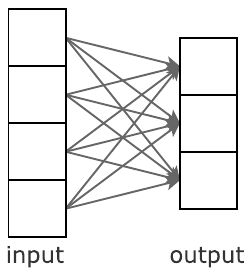
\includegraphics[height=5cm]{./statics/fully_connected.png}
    \caption{یک شبکه \gls{fully connected} با ۴ ورودی و ۳ خروجی}
\end{figure}

این لایه توسط رابطه زیر مدل می‌شود:
\begin{equation}
    y = f(W.x + b)
\end{equation}
که $x$ و $y$ بردارهایی از اعداد حقیقی هستند که به ترتیب متناظر با ورودی و خروجی
شبکه هستند. $W$ ماتریس وزن شبکه است که تعداد سطرهای آن برابر ابعاد ورودی و تعداد
ستون‌های آن برابر ابعاد خروجی است. همچنین $b$ بایاس شبکه است که عمکردی مانند عرض
از مبدا دارد و برداری از اعداد حقیقی با ابعادی برابر خروجی است. $f$ تابع
فعال‌سازی است که شبکه از آن استفاده می‌کند.

ورودی یک شبکه \gls{fully connected} تبدیل به برداری با ابعادی برابر با تعداد
نرون‌های خروجی می‌شود. در تئوری یک نرون خروجی می‌تواند حجم زیادی اطلاعات، در
صورتی که دقت محاسباتی به اندازه کافی باشد، را شامل شود. ولی در عمل معمولا هر
نرون یک ویژگی را فرا می‌گرد آن را نمایش می‌دهد. همچنین یک لایه با ابعادی پایین
می‌تواند در شبکه به عنوان یک تنگنا برای حجم اطلاعاتی که منتقل می‌شود ظاهر شود.

برای بسیاری از مسائل ابعاد خروجی به شدت از ابعاد ورودی کمتر است. در این شرایط
معمولا اندازه لایه‌های میانی برابر با اندازه‌ای ما بین تعداد نرون‌های ورودی و
خروجی قرار داده می‌شود. به این شکل اطلاعات در طول شبکه فشرده‌تر می‌شوند و فقط
اطلاعات مورد نیاز مسئله باقی می‌مانند.

\subsection{شبکه تماما همبند در موسیقی}
در \gls{mir} از شبکه‌های \gls{fully connected} به صورت گسترده استفاده می‌شود تا
یک تبدیل بر روی هر فرم موسیقی ورودی اعمال شود و ویژگی‌های مورد نیاز از آن
استخراج شود. به این منظور بر روی هر فرم \gls{spec} یک شبکه \gls{fully connected}
یک‌سان اعمال می‌شود. با قرار دادن تعدادی لایه \gls{fully connected} بر روی
\gls{spec} می‌تواند انتظار داشت شبکه فرا بگیرد که فرکانس‌های ورودی به فضای دیگر
منتقل کند که حل مسئله در آن ساده‌تر است. برای مثال در صورتی که مسئله تشخیص
\glspl{pitch} فعال در هر فرم است و شبکه به تعداد \glspl{pitch} مورد نظر خروجی
دارد، می‌توان انتظار داشت که شبکه یادبگیرد هر نرون خروجی را با یکی از
\glspl{pitch} مورد نظر متناظر کند.

همچنین با توجه شکل تعریف شبکه \gls{fully connected} واضح است که این شبکه در
مقابل تغییر در مکان یا مقیاس فرکانس‌ها حساس است. برای مثال در صورتی که مسئله
مورد نظر تشخیص \glspl{pitch} فعال در هر فرم باشد، تنها با تغییر جزئی در کوک ساز
مورد بررسی، شبکه خروجی کاملا متفاوت و نادرست تولید خواهد کرد. واضحا این
آسیب‌پذیری برای بسیاری از مسائل مطلوب نیست و باعث کاهش دقت جدی در سیستم نهایی
می‌شود. از همین جهت این ساختار بیشتر از قبل محبوبیت ساختارهایی مانند \gls{cnn} و
\gls{rnn} مورد استفاده قرار می‌گرفته است. همچنین شبکه‌های \gls{fully connected}
به علت قابلیت تحلیل بالاتر نسبت به سایر ساختارها، در سیستم‌هایی به علت محدودیت
\gls{dataset} و زیر ساخت محاسباتی به صورت \gls{e2e} آموزش داده نمی‌شود، مورد
استفاده قرار می‌گرفته‌اند.

\section{شبکه عصبی پیچشی}
\gls{cnn} اولین بار در سال ۱۹۸۸ معرفی شد ولی به علت محدودیت زیرساخت محساباتی در
زمان انتشار به محبوبیت زیادی دست نیافت. با این وجود امروزه یکی از مهمترین
ساختارهایی است که در \gls{dl} مورد استفاده قرار می‌گیرد و بسیاری از سیستم‌های
مطرح از آن‌ها استفاده می‌کنند.

\gls{cnn} نسبت به شبکه \gls{fully connected} مزایای بسیاری دارد. از مهم‌ترین این
مزایا شباهت نحوه عملکرد این شبکه‌ها به سیستم بنایی مغز انسان است. به عبارت دیگر
این ساختار به شدت برای پردازش عکس‌های دوبعدی و سه‌بعدی مناسب است و توانای
فراگیری و استخراج ویژگی‌های مجرد از عکس‌های ورودی را دارد. استفاده از \gls{max
pooling} که به صورت گسترده در \gls{cnn} استفاده می‌شود، به این شبکه‌ها مقاوت
نسبی در تغییر ابعاد ویژگی‌های ورودی می‌شود. همچنین با توجه ارتباطات تنک که در
\gls{CNN} استفاده می‌شود، این ساختار وزن‌های کمتری نسبت به شبکه \gls{fully
connected} دارد. همچنین این شبکه‌ها در طول فرآیند آموزش کمتر محو شدن گرادیان‌ها
رنج می‌برند که باعث دقت بالاتری در سیستم نهایی می‌شود. در نهایت این شبکه‌ها به
علت اشتراکی بودن وزن‌ها، قابلیت تعمیم بالاتری نیز دارند.

لایه \gls{convolution} دو بعدی را می‌توان توسط رابطه زیر مدل کرد:
\begin{equation}
    y^j = f(\sum_{k=0}^{K-1} W^{jk} \ast x^k + b^j)
\end{equation}
که $x^k$، $W^{jk}$، $b^j$ و $y^j$ همگی ماتریس‌هایی از اعداد حقیقی هستند. $x^k$
کانال $k$ام ورودی است. همچنین $y^j$ کانال $j$ام خروجی لایه است. $W^{jk}$ کرنلی
است که کانال $k$ام ورودی را به کانال $j$ام خروجی مرتبط می‌سازد. $b^j$ بایاس
متناظر با کانال $j$ام خروجی است. همچنین $\ast$ عملکرد \gls{convolution} است. در
نهایت $f$ تابع فعال‌ساز استفاده شده برای لایه است.

کرنل عملکرد \gls{convolution} همانند یک جارو بر روی کل ورودی حرکت می‌کنند و
خروجی را محسابه می‌کند. در نتیجه یک کرنل کوچک می‌تواند تبدیل ورودی به خروجی را
بگیرد و برای هر بخش از ورودی وزن‌هایی جدا استفاده نشود. به این عملکرد
اشتراک‌گذاری وزن‌ها نام دارد و باعث کاهش بسیار زیاد وزن‌های لایه می‌شود. در شکل
زیر نمونه از اعمال کرنل \gls{convolution} بر روی ورودی نمایش داده شده است.
\begin{figure}[ht]
    \centering
    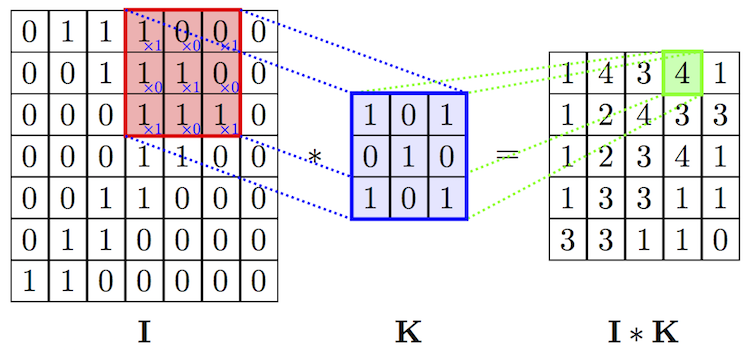
\includegraphics[height=5cm]{./statics/convolve_operator.png}
    \caption{نمونه‌ای از اعمال عملکرد \gls{convolution} بر روی ماتریس ورودی}
\end{figure}

به ازای یک ورودی داده شده، لایه \gls{convolution} با اعمال کرنل برروی بخش‌های
مختلف ورودی، میزان حضور الگوی متناظر با کرنل را در آن ناحیه بررسی می‌کند. در
نتیجه لایه \gls{convolution} بر خلاف لایه‌های \gls{fully connected} و \gls{rnn}
اطلاعات \gls{spatiality} را حفظ می‌کند. از این جهت به خروجی این لایه‌ها
\gls{feature map} می‌گویند.

با توجه به تعریف می‌توان گفت که لایه \gls{convolution} هم‌بستگی بین کرنل داده
شده و نقاط مختلف ورودی را اندازه‌گیری می‌کند. در طول فرآیند یادگیری، کرنل‌ها
الگوهایی که برای کاهش خطا مفید هستند را پیدا می‌کنند و فرا می‌گیرند. وقتی که
تعدادی از این لایه‌ها در ادامه هم قرار داده شوند، لایه‌های جلوتر می‌توانند از
\glspl{feature map} استخراج شده در لایه‌های قبل استفاده کنند تا ویژگی‌های سطح
بالاتری را اسخراج کنند. برای مثال در یک شبکه که با تصاویر مختلف به عنوان ورودی
آموزش دیده است، در لایه‌های اول هر کرنل مسئول اسخراج خطوط است و خطوط در زوایای
مخلف استخراج می‌شوند. لایه‌های بعدی می‌توانند از این خطوط استخراج شده استفاده
کنند تا شکل‌های ساده هندسی را شناسی کنند.

\subsection{لایه تجمع}
لایه‌های \gls{pooling} معمولا همراه با لایه‌های \gls{convolution} استفاده
می‌شوند تا ابعداد \glspl{feature map} تولید شده را کاهش دهند. لایه‌های تجمع با
اعمال یک تابع بر روی بخش‌های مختلف هر \gls{feature map} داده شده، سایز آن‌را
کاهش می‌دهند. نکته قابل توجه این است که لایه‌های \gls{pooling} بر روی تعداد
\gls{feature map} ورودی تاثیری ندارند و تنها ابعاد هر کدام از آن‌ها را به صورت
مستقل کاهش می‌دهند.

برای کاهش بعد معمولا از تابع بیشینه استفاده می‌شود. با استفاده از تابع بیشینه
فقط وجود یا عدم وجود یک ویژگی در هر محدوده مهم می‌شود. هرچه وجود یک ویژگی بیشتر
باشد، مقدار متناظر در \gls{feature map} بالاتر است. در نتیجه تابع بیشینه بیشترین
مقدار حضور را برای هر منطقه در نظر می‌گیرد و با مقادیر دیگر کاری ندارد. لایه
\gls{pooling} که از تابع بیشینه استفاده می‌کند با نام \gls{max pooling} شناخته
می‌شود. همچنین استفاده از لایه باعث افزایش مقاومت شبکه نسبت به تغییرات جزئی در
سایز اجسام ورودی می‌شود. شکل زیر نمونه‌ای از اعمال این لایه بر روی ورودی را نشان
می‌دهد.
\begin{figure}[ht]
    \centering
    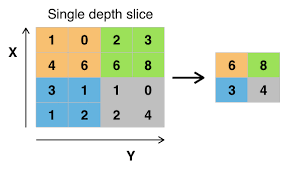
\includegraphics[height=5cm]{./statics/max_pooling.png}
    \caption{نمونه‌ای از اعمال \gls{max pooling} با سایز ۲در۲ بر روی ورودی}
\end{figure}

\subsection{شبکه عصبی پیچشی در موسیقی}
از لایه‌های \gls{convolution} دو بعدی معمولا برای استخراج ویژگی‌ها از \gls{spec}
ورودی استفاده می‌شود. از آن‌جایی که \gls{spec} نیز مانند عکس نمایشی دو بعدی
دارد، این لایه‌ها برای استخراج ویژگی از آن‌ها بسیار کارا هستند. همچنین با رسم
کرنل‌های استفاده شده می‌توان میزانی درک کرد که شبکه بر چه ویژگی‌های حساس شده است
و تلاش می‌کند چه ویژگی از ورودی را درک کند.

ابعاد کرنل‌های استفاده شده کاملا بستگی به مسئله مورد نظر دارد. اگر ابعاد کرنل
استفاده شده از الگوهای مورد نظر مسئله کوچک‌تر باشد، شبکه نمی‌تواند
\glspl{feature map} مناسب و با معنی تولید کند. برای مثال در مسئله تشخیص
\glspl{chord} در موسیقی ورودی کرنل باید به اندازه کافی بزرگ باشد تا بتواند تفاوت
\glspl{chord} ماژور با مینور را تشخیص دهد. از همین جهت در این مسائل استفاده از
کرنل‌های نسبتا بزرگی با سایز ۱۷در۵ رایج است. از طرفی دیگر، با افزایش سایز کرنل
استفاده شده، مقاوت شبکه در مقابل تغییرات جزئی در فرکانس‌های ورودی به شدت کاهش
می‌یابد. در نتیجه اگر هدف نهایی تشخیص الگوهای بسیار بزرگ در \gls{spec} ورودی
است، معمولا مناسب‌تر است که از یک \gls{cnn} چند لایه استفاده شود و در بین
لایه‌های \gls{convolution} از لایه‌های \gls{max pooling} استفاده شود. به این
ترتیب شبکه نسبت به تغییرات جزئی مقاوم خواهد بود و همچنین می‌تواند الگوهای بزرگ
را تشخیص دهد.

همچنین لایه‌های \gls{max pooling} به صورت گسترده در مسائل \gls{mir} استفاده
می‌شود. با کمک این لایه‌ها می‌توان مقاوت شبکه را در مقابل تغییرات جزئی در فرکانس
و کشش نت‌ها را بالا برد.

از لایه‌های \gls{convolution} یک بعدی نیز برای پردازش سیگنال‌های صوتی استفاده
می‌شود. با اعمال این لایه‌ها بر روی سیگنال‌های صوتی ضبط شده، شبکه می‌‌آموزد که
هر شکل تغییر در سیگنال ورودی با چه فرکانس‌هایی متناظر است و نیاز به محاسبه
\gls{spec} به صورت مستقل از بین می‌رود. همچنین این تبدیل به دست آمده، بر خلاف
موارد مانند \gls{stft}، توانایی تحلیل هارمونیک‌ها را نیز دارا هست.

\section{شبکه عصبی بازگشتی}
مغز انسان در هر لحظه فقط از داده‌ای که ورودی دریافت کرده استفاده نمی‌کنم. بلکه
از ورودی‌های قبلی هم استفاده می‌کند و بر اساس اجتماع این ورودی‌ها تصمیم می‌گیرد.
یا وقتی که متنی را مطالعه می‌کنید هر کلمه در ذهن با توجه به کلمات پیشین معنا
می‌شود و هر کلمه به صورت جدا تحلیل نمی‌شود. این رفتار را شبکه‌های \gls{fully
connected} یا \gls{cnn} نمی‌توانند نشان دهند. این ساختارها تنها می‌توانند یک
بردار ورودی با اندازه ثابت را پردازش کنند و همچنین خروجی با طول ثابت تولید کنند.
در نتیجه به ساختاری متفاوت که توانایی تحلیل دنباله‌ای از بردارها را داشته باشد و
خروجی به شکل دنباله‌ای از بردارها تولید کند حس می‌شود. \gls{rnn} می‌تواند یک
دنباله از بردارهای ورودی را در طول زمان پردازش کند و یک حافظه اطلاعاتی تا کنون
پردازش کرده است نگه‌دارد. این مفهوم اولین بار در سال ۱۹۸۲ توسط شبکه Hotfield
معرفی شد.

\gls{rnn} برای نگه‌داری اطلاعات ورودی‌های گذشته، یک خروجی متفاوت از خروجی اصلی
مدل دارند که نشان‌دهنده وضعیت داخلی مدل است و با نام وضعیت پنهان شناخته می‌شود.
در هر مرحله شبکه علاوه بر بردار ورودی، مقدار وضعیت پنهان تولید شده در مرحله قبل
را زیر دریافت می‌کند. در نتیجه شبکه در تئوری، می‌تواند به تمام اطلاعات قبلی نیز
دسترسی داشته باشد و از آن‌ها برای تصمیم گیری استفاده کند. این ساختار را توسط
روابط زیر می‌توان مدل کرد:
\begin{equation}
    y_t = f_{out}(Vh_t)
\end{equation}
\begin{equation}
    h_t = f_h(Ux_t + Wh_{t-1})
\end{equation}

در روابط بالا $f_{out}$ تابع فعال‌ساز خروجی اصلی مدل است. $f_h$ تابع فعال‌ساز
وضعیت پنهان است که معمولا از تابع تانژانت هیپربولیک یا ReLU برای آن استفاده
می‌شود. $x_t$ ورودی شبکه در زمان $t$ است. همچنین $y_t$ و $h_t$ به ترتیب خروجی
مدل و وضعیت پنهان شبکه در زمان $t$ هستند. همچنین $V$، $U$ و $W$ ماتریس وزن‌های
شبکه هستند که در طول فرآیند آموزش مقدار آن‌ها در جهت کاهش خطا تغییر می‌کند. برای
تمایز این ساختار با سایر اعضای خانواده \gls{rnn}، به این ساختار شبکه عصبی
بازگشتی ساده نیز می‌گویند.

برای درک بهتر \gls{rnn} می‌توان آن را با استفاده از شبکه \gls{fully connected}
تحلیل کرد. می‌توان فرض کرد که ابتدا ورودی شبکه توسط یک شبکه \gls{fully
connected} با وزن‌های $U$ بررسی می‌شود و مقدار $z$ از آن تولید می‌شود. سپس وضعیت
مخفی تولید شده در مرحله قبل، که می‌توان مثل هر بردار ورودی دیگر با آن برخورد
کرد، توسط یک شبکه \gls{fully connected} دیگر با ماتریس وزن $W$ پردازش می‌شود.
خروجی این شبکه با $z$ جمع می‌شود و پس از عبور از یک تابع فعال‌سازی مقدار $h_t$
به دست می‌آید. در نهایت $h_t$ به شبکه دیگری داده می‌شود که ماتریس وزن‌های آن $V$
است و خروجی نهایی به دست می‌آید. پس می‌توان هر \gls{rnn} را مجموعه‌ای از سه شبکه
\gls{fully connected} دانست. شکل زیر این متلب را به خوبی نشان می‌دهد.
\begin{figure}[ht]
    \centering
    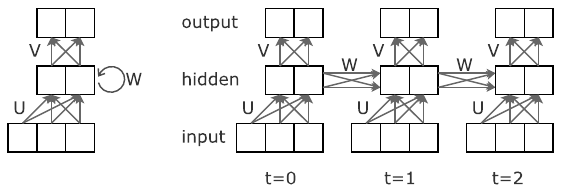
\includegraphics[height=4cm]{./statics/rnn_unfolding.png}
    \caption{ارتباط \gls{rnn} با شبکه‌های \gls{fully connected}}
\end{figure}

این نگاه به \gls{rnn} شیوه آموزش این شبکه‌ها را نیز واضح می‌کند. به همان صورت که
نشان داده شد، می‌توان \gls{rnn} را به صورت دنباله‌ای پشت‌سر هم از شبکه‌های
\gls{fully connected} در نظر گرفت. در نتیجه برای آموزش کافی است که حالت باز شده
شبکه را در نظر گرفت و در هر مرحله گرادیان خطا را برای هر ماتریس وزن توسط
\gls{backpropagation} محاسبه کرد. از آن‌جا که هر وزن در مقدار خطا در چندین مرحله
تاثیر دارد، در زمان به روز رسانی وزن‌ها از مجموع گرادیان‌های به دست آمده استفاده
می‌شود. این نسخه از \gls{backpropagation} به \gls{bptt} معروف است.

\gls{rnn} تلاش می‌کند مدلی برای محاسبه احتمال زیر ارائه دهد:
\begin{equation}
    P(y_t | x_{t-k}, ..., x_t)
\end{equation}
این دقیقا هدفی است که \gls{hmm} نیز تلاش می‌کند به آن برسد. با این وجود
\gls{hmm} از n حالت مختلف استفاده می‌کند. در حالی که \gls{rnn} از یک بردار
پیوسته از اعداد حقیقی استفاده می‌کند. در نتیجه حداقل در تئوری \gls{rnn}، در صورت
وجود داده آموزشی کافی، می‌تواند خیلی بهتر این احتمال را تقریب بزند.

\subsection{شبکه عصبی بازگشتی دوجهته}
یکی از مشکلات \gls{rnn} این است که در هر مرحله برای تصمیم‌گیری تنها به اطلاعاتی
دسترسی داریم که پیش از این در دنباله ورودی‌ها ظاهر شده‌اند. برای بعضی از مسائل
این محدودیت می‌تواند مشکل‌ساز باشد. برای مثال در مسئله برچسب‌زنی اجزای کلام،
داشتن کلماتی که در ادامه در جمله ظاهر می‌شوند، برای تشخیص نقش کلمه‌ای که در لحظه
به شبکه داده شده است می‌تواند بسیار به دقت مدل کمک کند.

برای حل این مشکل می‌توان از دو \gls{rnn} مجزا استفاده کرد. به یکی از این شبکه‌ها
دنباله ورودی‌ها به صورت معکوس داده می‌شود. سپس از خروجی هر دو شبکه برای
نتیجه‌گیری با هم استفاده می‌شود. این ساختار را می‌توان توسط روابط زیر مدل کرد:
\begin{equation}
    y_t = f_{out}(Vh_t + V^\prime h_t^\prime)
\end{equation}
\begin{equation}
    h_t = f_h(Ux_t + Wh_{t-1})
\end{equation}
\begin{equation}
    h_t^\prime = f_h(U^\prime x_{T - t} + W^\prime h_{t-1}^\prime)
\end{equation}
که $T$ طول دنباله ورودی است. با این ساختار در هر مرحله شبکه به تمام اطلاعات
دنباله ورودی دسترسی دارد و می‌تواند از آن‌ها برای تصمیم‌گیری استفاده کند.

\subsection{حافظه طولانی کوتاه-مدت}
یکی مشکلات اصلی شبکه عصبی بازگشتی ساده، محو شدن گرادیان‌ها است. در نتیجه شبکه با
این که در تئوری باید بتواند روابط با هر طولی را بین بردارهای ورودی یادبگیرد، ولی
در عمل به علت محو شدن گرادیان‌ها شبکه فقط روابط نزدیک را فرا می‌گیرد. \gls{lstm}
دقیقا با این مشکل در ذهن طراحی و به خاطر ساختار دروازه‌هایی که استفاده می‌کند
می‌تواند تا مقدار خوبی این مشکل را حل کند.

خصوصیت اصلی \gls{lstm} استفاده از یک خروجی مخفی دیگر، علاوه بر وضعیت پنهان، به
اسم وضعیت سلول است. این شبکه با استفاده از سه دروازه ورودی، فراموشی و خروجی
کنترل می‌کند چه اطلاعتی به این خروجی اضافه و کم شود. رفتار این دروازه‌ها توسط
روابط زیر بیان می‌شود:
\begin{equation}
    f_t = \sigma(W_f [h_{t-1},x_t] + b_f)
\end{equation}
\begin{equation}
    i_t = \sigma(W_i [h_{t-1},x_t] + b_i)
\end{equation}
\begin{equation}
    \tilde{C_t} = tanh(W_C [h_{t-1}, x_t] + b_C)
\end{equation}
\begin{equation}
    C_t = f_t * C_{t-1} + i_t * \tilde{C_t}
\end{equation}
\begin{equation}
    O_t = \sigma(W_O [h_{t-1},x_t] + b_O)
\end{equation}
\begin{equation}
    h_t = O_t * tang(C_t)
\end{equation}
که $C_t$ وضعیت سلول است. این خروجی در کنار وضعیت پنهان، $h_t$، وظیفه نگهداری
اطلاعات گذشته را دارند. همچنین همان‌طور که در روابط نشان داده شده است هر دروازه
وزن‌ها و بایس خود را دارد که در طی فرآیند آموزش فرامی‌گیرد چه تغییری در وضعیت
سلول باید ایجاد کند. شکل زیر نمایی از یک سلول \gls{LSTM} را نشان می‌دهد.
\begin{figure}[ht]
    \centering
    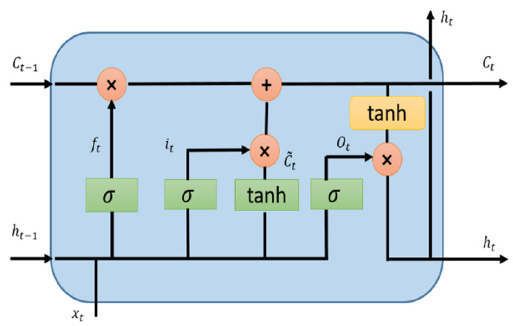
\includegraphics[height=4.5cm]{./statics/lstm_cell.png}
    \caption{نمایی از یک سلول \gls{LSTM}}
\end{figure}

\subsection{واحد دروازه‌بندی‌شده بازگشتی}
یکی از مشکلات \gls{lstm} پیچیدگی زیاد ساختار و پارامترهای زیادی است که در طول
آموزش نیاز است تا فراگرفته شوند. این پیچیدگی باعث سربار محاسباتی بالا این ساختار
می‌شود. برای حل این مشکلات \gls{gru} پیشنهاد داده شد. \gls{GRU} همانند
\gls{LSTM} از ساختار دروازه‌ها استفاده می‌کند تا کنترل کند چه اطلاعاتی از مرحله
نگه‌داری شوند. با این تفاوت که این ساختار بجای سه دروازه از دو دروازه استفاده
می‌کند. در \gls{gru} دروازه‌های ورودی و فراموشی با هم ترکیب شده‌اند و در قالب یک
دروازه عمل می‌کنند. همچنین این ساختار وضعیت سلول را با وضعیت مخفی ترکیب کرده است
و یک خروجی اضافه از مدل حذف شده است.

این سبک سازی ساختار باعث شده است سربار محاسبه به شکل قابل محسوسی کاهش پیدا کند و
آموزش شبکه ساده‌تر شود. این مزیت باعث محبوبت این مدل برای بسیاری از مسائل شده
است. \gls{gru} را می‌توان با استفاده از روابط زیر مدل کرد:
\begin{equation}
    z_t = \sigma(W_z [h_{t-1},x_t])
\end{equation}
\begin{equation}
    r_t = \sigma(W_r [h_{t-1},x_t])
\end{equation}
\begin{equation}
    \tilde{h_t} = tanh(W [r_t * h_{t-1}, x_t])
\end{equation}
\begin{equation}
    h_t = (1 - z_t) * h_{t-1} + z_t * \tilde{h_t}
\end{equation}

هیچ مدرک محکمی برای برتری قطعی هیچ یک از ساختارهای \gls{GRU} و \gls{LSTM} نسبت
به دیگری وجود ندارد. از طرفی \gls{gru} به علت داشتن پارامترهای کمتر، بار
محاسباتی کمتری دارد. ولی از طرفی دیگر، در صورت وجود داده کافی برای آموزش،
\gls{lstm} به نتایج بهتری می‌توان دست پیدا کند. در نتیجه انتخاب بین این دو
ساختار وابسطه به مسئله و میزان داده آموزشی موجود است.

\subsection{شبکه بازگشتی عصبی در موسیقی}
همگونه که بحث شد، \gls{rnn} را می‌توان یک شبکه \gls{fully connected} در نظر گرفت
که علاوه بر بردار ورودی اصلی، اطلاعات کد شده قبلی را نیز به عنوان ورودی دریافت
می‌کند. در نتیجه این شبکه نیز همانند شبکه \gls{fully connected} در مقابل تغییرات
جزئی در مکان و یا مقیاس فرکانس‌ها ورودی آسیب پذیر است. در نتیجه استفاده مستقیم
این ساختار بر روی \gls{spec} زیاد رایج نمی‌باشد و معمولا توصیه می‌شود ورودی این
شبکه \glspl{feature map} باشد که در مراحل قبل استخراج شده‌اند. برای مثال می‌توان
با کمک \gls{cnn} از روی \gls{spec} \glspl{feature map} استخراج شود و خروجی به یک
\gls{rnn} داده شود.

همچنین اندازه بردار وضعیت مخفی استفاده شده در مدل جز \glspl{hyper parameter} پر
اهمیت می‌باشد. تمام اطلاعات مورد نیاز از نمونه‌های گذشته باید در قالب این بردار
به مراحل بعدی منتقل شود. در نتیجه در صورتی که این بردار به اندازه کافی بزرگ
نباشد، تمام اطلاعات مورد نیاز نمی‌توانند منتقل شوند و دقت مدل کاهش خواهد یافت.
معمولا این مقدار بین اندازه بردارهای ورودی و خروجی انتخاب می‌شود و پس از آن با
انجام آزمایش‌های پی‌در‌پی تلاش می‌شود تا اندازه مناسب آن مشخص شود.

همچنین ماهیت مسئله به انتخاب این مقدار می‌تواند کمک کند. برای مثال تشخیص شروع
نت‌ها تنها توسط چند فرم گذشته ممکن هست و فرم‌های عقب‌تر اطلاعات چندان بیشتری در
اختیار مدل نمی‌گذارند. در نتیجه در این مسئله می‌توان اندازه بردار وضعیت مخفی را
کوتاه‌تر کرد. از طرفی در مسئله‌ای مانند تشخیص \glspl{chord} فعال نیاز به
\glspl{chord} فعال گذشته است، در نتیجه به بردار وضعیت مخفی طولانی‌تری نیاز است.

در بسیاری از مسائل حوزه \gls{mir} داشتن اطلاعات بردارهای ورودی آینده، می‌تواند
دقت سیستم را به شکل قابل توجهی افزایش دهد. مثلا در مسئله تشخیص شروع نت‌ها در
صورتی که فرم‌های آینده نیز همراه فرم‌های گذشته به مدل داده شود، دقت به شکل
محسوسی افزایش می‌یابد. در این مسائل توصیه می‌شود از ساختار \gls{brnn} به شدت
توصیه می‌شود و می‌تواند تاثیر محسوسی بر روی دقت سیستم داشته باشد.

\section{روش‌های عادی‌سازی}
\gls{normalization} یکی از بحث‌هایی در \gls{dl} است که در سال‌های اخیر بسیار
مطالعه قرار گرفته است. استفاده از \gls{normalization} در شبکه مزایای بسیاری دارد
که محبوبیت آن‌ها را به خوبی توجیح می‌کند. به کمک این روش‌ها هر ویژگی ورودی شبکه
مقدارهای عددی در بازه مشابه دارند. به این ترتیب شبکه به ویژگی‌هایی که صرفا مقدار
عددی بالاتری دارند ولی ارزش بیشتری ندارند متمایل نمی‌شود. همچنین این روش‌ها با
تغییر توزیع احتمالی خروجی هر لایه، باعث آموزش بهتر شبکه می‌شوند و مدل نهایی از
دقت بالاتری برخورددار خواهد بود. همچنین با کنترل مقدار گرادیان‌ها از محو شدن یا
انفجار گرادیان‌ها جلوگیری می‌کنند و آموزش شبکه را سرعت می‌بخشند. همچنین این
روش‌ها تا حدی قابلیت تعمیم شبکه را افزایش می‌دهند و از \gls{overfit} جلوگیری
می‌کنند.

روش‌های مختلفی برای اعمال \gls{normalization} در \gls{dl} پیشنهاد شده است که هر
کدام مزایا و معایب خود را دارند و با توجه به ساختار شبکه و مسئله باید روش مناسب
انتخاب شود. در ادامه به بررسی سه روش پرطرفدارتر می‌پردازیم.

\subsection{عادی‌سازی دسته‌ای}
\gls{batch normalization}\cite{ioffe2015batch} از اولین روش‌هایی بود که برای
اعمال \gls{normalization} در \gls{nn} پیشنهاد داده شود. در \gls{batch
normalization} خروجی هر لایه در طول دسته داده شده به شبکه \gls{normalization}
می‌کند. این روش به ازای هر ویژگی در دسته داده شده، میانگین و واریانس ویژگی را
محاسبه می‌کند. سپس میانگین را از خروجی لایه کم می‌کند و نتیجه را به واریانس
تقسیم می‌کند. عملکرد این رابطه را می‌توان توسط روابط زیر مدل کرد:
\begin{equation}
    \mu_j := \frac{1}{m} \sum_{i=1}^{m}x_{ij}
\end{equation}
\begin{equation}
    \sigma_j^2 := \frac{1}{m} \sum_{i=1}^{m}(x_{ij} - \mu_j)^2
\end{equation}
\begin{equation}
    \hat{x_{ij}} := \frac{x_{ij} - \mu_j}{\sqrt{\sigma_j^2 + \epsilon}}
\end{equation}
\begin{equation}
    y_{ij} := \gamma_j \hat{x_{ij}} + \beta_j
\end{equation}
که $m$ اندازه دسته است. $x_{ij}$ ویژگی $j$ام از $i$امین نمونه در دسته است.
همچنین $\mu_j$ و $\sigma_j^2$ به ترتیب میانگین و واریانس ویژگی $j$ام هستند. در
نهایت $\gamma_j$ و $\beta_j$ پارامترهای \gls{batch normalization} هستند که در
طول فرآیند آموزش فراگرفته می‌شوند. نیاز به وجود این پارامترها از آن‌جا می‌آید که
بعضی از ویژگی‌ها در صورتی که میانگین و یا واریانسی متفاوت با توضیع نرمال
استاندارد داشته باشند، شبکه می‌تواند نتایج بهتری را تولید کند. از این جهت با کمک
این پارامترها می‌توان میانگین و واریانس این ویژگی‌ها را با توجه به نیز شبکه
تغییر داد.

\gls{batch normalization} علارقم نشان دادن نتایج بسیار عالی دو ایراد مهم دارد.
اولین مشکل نیاز این روش به داشتن دسته‌ای با اندازه بزرگ‌تر از یک است. اگر اندازه
دسته داده شده برابر یک باشد، یا به عبارتی در هر مرحله تنها یک نمونه به شبکه
آموزش داده شود، واریانس محاسبه شده برابر صفر می‌شود که عملکرد لایه را با مشکل
مواجه می‌کند. همچنین برای دسته‌هایی با اندازه کوچک مقادیر محاسبه شده قابل
اطمینان نیستند و می‌تواند در فرآیند آموزش مشکل ایجاد کنند. همچنین در \gls{rnn}
با توجه به این که هر مرحله، از آماره‌های متفاوتی تبعیت می‌کنند، در هر مرحله باید
\gls{batch normalization} به صورت جدا محاسبه شود که باعث پیچیدگی بیش از حد مدل
می‌شود.

\subsection{عادی‌سازی وزنی}
\gls{weight normalization}\cite{salimans2016weight} بر خلاف \gls{batch
normalization} بر اساس \gls{normalization} وزن‌های شبکه کار می‌کند. این روش هر
ماتریس وزن شبکه را با یک ماتریس جدید، $V$، و یک بردار دیگر، $g$، جایگزین می‌کند.
ماتریس وزن اصلی توسط رابطه زیر بدست می‌آید:
\begin{equation}
    W := \frac{g}{\parallel V \parallel} V
\end{equation}

به این ترتیب جهت ماتریس وزن‌ها توسط ماتریس $V$ بیان می‌شود و اندازه این ماتریس
توسط $g$ بیان می‌شود. حال در طول آموزش شبکه بجای آموختن، $W$، مقادیر $V$ و $g$
را می‌آموزد. این جداسازی نشان داده شده است که سرعت آموزش شبکه را افزایش می‌دهد و
تاثیرات مانند \gls{batch normalization} دارد. ولی وابستگی به اندازه دسته ورودی
شبکه از بین می‌رود و می‌توان از دسته‌هایی با اندازه کوچک و حتی یک استفاده کرد.
همچنین این ساختار بر خلاف \gls{batch normalization} به سادگی بر روی \gls{rnn}
قابل اعمال است.

\subsection{عادی‌سازی لایه‌ای}
\gls{layer normalization}\cite{ba2016layer} یک روش \gls{normalization} دیگر است
که تلاش می‌کند مشکلات \gls{batch normalization} را حل کند. در این روش بر خلاف
\gls{batch normalization} که ویژگی‌ها در طول دسته داده شده \gls{normalization}
می‌شوند، ویژگی‌ها در طول ویژگی‌های دیگر \gls{normalization} می‌شوند. با توجه به
روابط زیر و مقایسه آن‌ها با روابط \gls{batch normalization} تفاوت این دو روش به
خوبی نشان داده می‌شود.
\begin{equation}
    \mu_i := \frac{1}{m} \sum_{j=1}^{m}x_{ij}
\end{equation}
\begin{equation}
    \sigma_i^2 := \frac{1}{m} \sum_{j=1}^{m}(x_{ij} - \mu_i)^2
\end{equation}
\begin{equation}
    \hat{x_{ij}} := \frac{x_{ij} - \mu_i}{\sqrt{\sigma_i^2 + \epsilon}}
\end{equation}
$m$ تعداد ویژگی‌های داخل هر نمونه دسته است و $\mu_i$ و $\sigma_i^2$ به ترتیب
میانگین و واریانس ویژگی‌ها در نمونه $i$ام دسته هستند.

این روش دیگر وابستگی به اندازه دسته داده شده با شبکه ندارد. در نتیجه از
دسته‌هایی با هر اندازه‌ای می‌توان استفاده کرد. همچنین این روش بر روی \gls{rnn}
نیز نتایج بسیار رضایت بخشی نشان داده است.

\section{شبکه پیچشی زمانی}
در مسائلی که دادگان به صورت دنبالی‌ای از بردارها هستند، به صورت سنتی \gls{rnn}
ساختار اصلی مورد استفاده هستند. این شبکه تئوری می‌تواند اطلاعات با هر طولی از
گذشته را به خاطر بسپارد و از آن‌ها برای نتیجه گیری در هر مرحله استفاده کند. با
این وجود این ساختار مشکلات بسیاری دارد که باعث تحقیقات گسترده بر روی ساختارهای
جایگزین شده است. این شبکه‌ها از به شدت از مشکل محو شدن گرادیان‌ها رنج می‌برند و
حتی ساختاری مانند \gls{LSTM} نیز که برای حل این چالش طراحی شده است نیز برای
دنباله‌های بسیار طولانی همچنان از این مشکل تا حدی رنج می‌برد. از طرفی دیگر
\gls{rnn} به صورت ماهیتی قالیت موازی‌سازی را دارا نیستند. در این شبکه در هر
مرحله حتما خروجی شبکه محاسبه شده باشد تا بتوان محاسبات را پیش برد. به عبارتی
دیگر برای دنباله‌ای به طول هزار، باید هزار مرحله به صورت پشت سر هم محاسبه شوند و
نمی‌توان آن‌ها را همزمان انجام داد. همچنین این ساختارها حافظه بسیار زیادی در طول
آموزش نیاز دارند که آموزش آن‌ها با دنباله‌های طولانی را با مشکلات جدی می‌تواند
رو به رو کند.

\gls{tcn} به عنوان یک جایگزین برای \gls{rnn} با هدف حل مشکلات آن‌ها معرفی
شد\cite{bai2018empirical}. همان گونه که از اسم این ساختار مشخص است، این شبکه
کاملا بر اساس \gls{cnn} است. با این وجود با توجه به شکل قرار گیری لایه‌ها
محدودیت \gls{cnn} در پردازش داده‌های دنباله‌ای بر روی آن اعمال نمی‌شود.

این شبکه حاصل قرار گیری تعدادی لایه \gls{convolution} یک بعدی پشت سر هم است.
برای جلوگیری از تغییر طول دنباله ورودی، در هر مرحله به ابتدای بردار ورودی به
تعداد اندازه کافی بردارهای تمام صفر اضافه می‌شود. دلیل این که این بردارها فقط به
ابتدای دنباله اضافه می‌شود این در هر مرحله شبکه‌ برای پیشبینی فقط باید امکان
استفاده از اطلاعات گذشته را داشته باشد. در صورتی که این محدودیت در مسئله وجود
نداشته باشد، می‌توان با افزودن این بردار‌های تماما صفر به دو انتهای دنباله، به
شبکه این قابلیت را داد که از اطلاعات آینده نیز استفاده کند.

با قرار دادن تنها لایه‌های \gls{convolution} عادی پشت سر هم، هر نرون خروجی تنها
دامنه‌ی دید خطی‌ای از تعداد لایه‌ها را می‌تواند داشته باشد. در نتیجه اگر هر نرون
برای عملکرد صحیح به دامنه دید بالایی نیاز داشته باشد، نیاز است تعداد لایه‌ها
افزایش داده شود که منجر به پیچیدگی مدل و کاهش دقت و سخت‌تر شدن فرآیند آموزش
می‌شود. برای حل این مشکل پیشنهاد شد که از \gls{dilated convolution} به جای
\gls{convolution} ساده استفاده شود.

در \gls{dilated convolution} درایه‌های کرنل از یک دیگر فاصله دارند و کاملا به یک
دیگر متصل نیستد. به عبارتی دیگر با وجود این که اندازه کرنل‌ها تغییر نکرده است
ولی دامنه دید افزایش خواهد یافت. \gls{dilated convolution} را می‌توان توسط رابطه
زیر مدل کرد:
\begin{equation}
    F(s) = (x *_d f) = \sum_{i=0}^{k-1} f(i) x_{s-di}
\end{equation}
که $x$ دنباله ورودی است و $f$ کرنل استفاده شده است که طولی برابر $k$ دارد. $s$
عضوی از دنباله ورودی است که می‌خواهیم \gls{convolution} را بر روی آن اعمال کنیم.
$d$ نیز ضریب باز شدن فیلتر است. به این ترتیب برای افزایش دامنه دید هر نرون کافی
هست که در لایه $i$، مقدار $d$ را برابر $2^{i-1}$ قرار داده شود تا دامنه دید
نسبتی نمایی با تعداد لایه‌ها پیدا کند. شکل زیر به خوبی این شکل این ارتباطات را
نمایش می‌دهد.
\begin{figure}[ht]
    \centering
    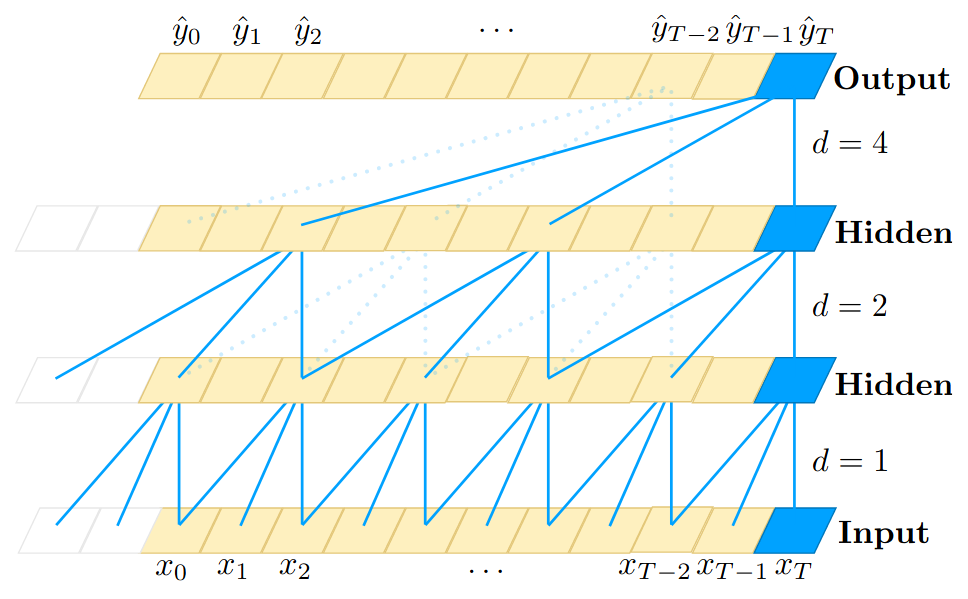
\includegraphics[height=7cm]{./statics/tcn_connections.png}
    \caption{شکل ارتباطات در \gls{tcn}}
\end{figure}

برای این که جریان گرادیان‌ها در این ساختار بهتر شود، از ارتباطهای رزیدوال
استفاده می‌شود. در هر واحد رزیدوال استفاده شده دو لایه \gls{dilated convolution}
وجود دارد که از تابع ReLU به عنوان تابع فعال‌سازی استفاده می‌کنند. بعد از هر
لایه یک لایه dropout وجود دارد که از \gls{overfit} شبکه جلوگیری کند. همچنین برای
\gls{normalization} در هر \gls{dilated convolution} از \gls{weight
normalization} استفاده می‌شود. با توجه به این که ممکن است تعداد ویژگی‌های ورودی
با خروجی هر واحد متفاوت باشد، برای اعمال ارتباط رزیدوال در صورت نیاز بر ورودی یک
\gls{convolution} یک بعدی اعمال می‌شود تا تعداد ویژگی‌ها برابر خروجی شود.

این ساختار بر خلاف \gls{rnn} می‌تواند به صورت موازی آموزش داده شود. همچنین به
علت این که مسیری که گرادیان باید در آن حرکت کند، به شدت کوتاه‌تر است، در نتیجه
محو شدن گرادیان‌ها خیلی کمتر رخ می‌دهد و شبکه می‌توان بدون هیچ مشکلی آموزش
ببیند. در مقایسه با \gls{rnn} نیز این ساختار مصرف حافظه بسیار کمتری دارد. با این
وجود این ساختار می‌تواند تنظیم شود که در هر مرحله از اطلاعات گذشته و آینده با هر
فاصله‌ای استفاده کند و مانند \gls{rnn} می‌تواند به راحتی با دادگان دنباله‌ای
استفاده شود. در آزمایشاتی که انجام شد \cite{bai2018empirical} نشان داده شد که
این ساختار می‌تواند از ساختارهای مانند \gls{lstm} و \gls{gru} نتایج بهتری به دست
آورد.

\section{مبدل}
برای ترجمه یک دنباله از بردارهای ورودی به دنباله‌ای به طول متفاوت از بردارهای
خروجی به صورت سنتی از \gls{rnn} استفاده می‌شود. در این سیستم‌ها معمولا یک
\gls{rnn} ابتدا کل دنباله ورودی را در قالب یک بردار کد می‌کند و سپس یک \gls{rnn}
دیگر این بردار را گرفته و دنباله‌ی خروجی را با توجه به آن تولید می‌کند. این
ساختار نیز از تمام مشکلات \gls{rnn} رنج می‌برد. همچنین با توجه به محدودیت یک
بردار در انتقال کل مفهوم دنباله ورودی، نیاز به یک ساختار مناسب‌تر کاملا محسوس
بود.

\gls{transformer} یکی از ساختارهای جایگزینی است که برای مسائل تبدیل دنباله به
دنباله پیشنهاد داده شد \cite{vaswani2017attention}. این ساختار تنها با استفاده
از میکانیک \gls{attention} و لایه‌های \gls{fully connected} که بر روی هر بردار
ورودی به صورت جداگانه اعمال می‌شوند، توانست موفقیت‌های بسیاری در حوزه‌های مختلف،
مخصوصا پردازش زبان طبیعی، به دست آورد.

در این ساختار ابتدا دنباله ورودی $(x_1, ..., x_n)$ به بخش \gls{encoder} مدل داده
می‌شود تا تبدیل به دنباله $(z_1, ..., z_n)$ شود. سپس بخش \gls{decoder} تلاش
می‌کند دنباله خروجی $(y_1, ..., y_m)$ را با استفاده از $z$ تولید کنید. این بخش
در مرحله با دریافت کل $z$ و آخرین عضو تولید شده از $y$ عضو بعدی دنباله $y$ را
تولید می‌کند. در شکل ساختار شبکه \gls{transformer} نشان داده شده است.
\begin{figure}[ht]
    \centering
    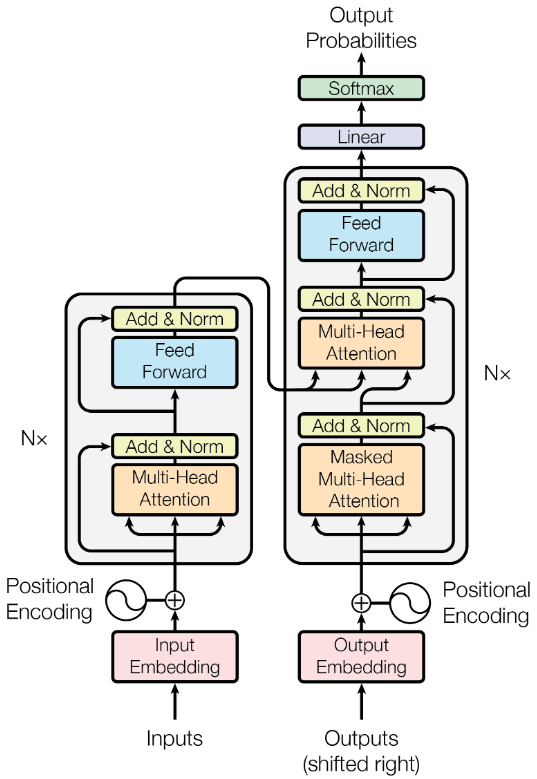
\includegraphics[height=12cm]{./statics/transformers_architecture.png}
    \caption{معمار استفاده شده در \gls{transformer}}
\end{figure}

\subsection{دقت ضرب نقطه‌ای متناسب شده}
ورودی \gls{scaled dot-product attention} شامل بردارهای جستار و کلیدهایی به ابعاد
$d_k$ و همچنین بردارهای ورودی با ابعاد $d_v$ است. به ازای هر بردار جستار، ضرب
نقطه‌ای آن با تمام بردارهای کلید محاسبه می‌شود و نتیجه بر $\sqrt{d_k}$ تقسیم
می‌شود. سپس بر روی مقادیر به دست آمده تابع $softmax$ اعمال می‌شود تا میزان تاثیر
هر بردار ورودی محاسبه شود.

برای سرعت بخشیدن به محاسبات کل جستارهای ورودی به شکل یک ماتریس $Q$ در نظر گرفته
می‌شود. بردارهای ورودی و کلیدها نیز به شکل ماتریس‌های $V$ و $K$ در نظر گرفته
می‌شوند. در نتیجه با استفاده از رابطه زیر می‌توان مقدار \gls{scaled dot-product
attention} را محاسبه کرد.
\begin{equation}
    softmax(\frac{QK^T}{\sqrt{d_k}})V
\end{equation}

\subsection{دقت چند سر}
در \gls{multi-head attention} بجای اعمال تنها یک \gls{scaled dot-product
attention}، ابتدا جستارها، کلیدها و بردارهای ورودی توسط $h$ تبدیل خطی مختلف به
بردارهایی به ترتیب با ابعاد $d_k$، $d_k$ و $d_v$ تبدیل می‌شوند. سپس بر روی $h$
مجموعه جستارها، کلیدها و ورودی‌های به دست آمده، $h$، \gls{scaled dot-product
attention} مختلف اعمال می‌شود. مقادیر به دست آمده سپس در کنار هم قرار می‌گیرند و
وسط تبدیل خطی دیگر به برداری با ابعاد خروجی تبدیل می‌شوند. به این ترتیب مدل در
هر مرحله می‌تواند به بخش‌های مختلف توجه کند و بر اساس مجموع این توجه‌های به دست
آمده خروجی را تولید کند. همچین قابل توجه است که تبدیل‌های خطی اعمال شده نیز در
طول فرآیند آموزش فراگرفته می‌شوند. شکل زیر به خوبی شیوه اعمال \gls{multi-head
attention} را نشان می‌دهد.
\begin{figure}[ht]
    \centering
    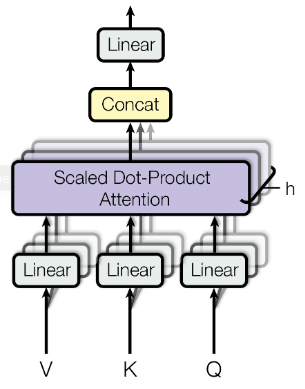
\includegraphics[height=6cm]{./statics/multi_head_attention.png}
    \caption{شیوه اعمال \gls{multi-head attention}}
\end{figure}

\subsection{بخش‌های رمزگذار و رمزگشا}
بخش \gls{encoder} شامل شش قسمت کاملا مشابه است. هر قسمت از دو لایه تشکیل شده
است. لایه اول \gls{multi-head attention} و لایه دوم یک شبکه \gls{fully
connected} است که بر روی هر بردار دنباله به صورت جداگانه اعمال می‌شود. همچنین هر
کدام از این لایه‌ها از ارتباط رزیدوال استفاده می‌کند و \gls{layer normalization}
بهره می‌برند.

بخش \gls{decoder} نیز از شش قسمت کاملا مشابه تشکیل شده است. هر قسمت شامل دو لایه
\gls{multi-head attention} و یک شبکه \gls{fully connected} است. لایه
\gls{multi-head attention} اول مقادیر دنباله خروجی‌ای که تولید شده است را به
عنوان ورودی می‌گیرد. \gls{multi-head attention} دوم علاوه بر خروجی لایه قبل به
کل خروجی بخش \gls{encoder} دست‌رسی دارد. در \gls{decoder} نیز مانند
\gls{encoder} در تمام لایه‌ها از ارتباط رزیدوال و \gls{layer normalization}
استفاده شده است.